\synctex=1
\documentclass[a4paper,11pt,svgnames]{book}

\usepackage[utf8x]{inputenc}
\usepackage{mathtools}
\usepackage{thesis}
\usepackage{calc}
\usepackage{gensymb}
\usepackage{xspace}
\usepackage{csquotes}
\usepackage{amsfonts}
\usepackage[algochapter]{algorithm2e}
\setlength{\marginparwidth}{2cm}
\setlength{\voffset}{-0.25in}
\setlength{\parskip}{0.1in}

%\includeonly{5-architecture}
%\includeonly{6-use-case}

%\usepackage{draftwatermark}
%\SetWatermarkScale{4}
\usepackage{subfig}
 \usepackage{listings}
  \usepackage{courier}
 \lstset{
 		 basicstyle=\footnotesize\ttfamily,
         numbers=none,               % Ort der Zeilennummern
         numberstyle=\tiny,          % Stil der Zeilennummern
         %stepnumber=2,               % Abstand zwischen den Zeilennummern
         numbersep=5pt,              % Abstand der Nummern zum Text
         tabsize=2,                  % Groesse von Tabs
         extendedchars=true,         %
         breaklines=true,            % Zeilen werden Umgebrochen
         keywordstyle=\color{red},
    	 frame=single,         
 %        keywordstyle=[1]\textbf,    % Stil der Keywords
 %        keywordstyle=[2]\textbf,    %
 %        keywordstyle=[3]\textbf,    %
 %        keywordstyle=[4]\textbf,   \sqrt{\sqrt{}} %
         stringstyle=\color{white}\ttfamily, % Farbe der String
         showspaces=false,           % Leerzeichen anzeigen ?
         showtabs=false,             % Tabs anzeigen ?
         belowcaptionskip=5pt, 
         xleftmargin=2em, 
         xrightmargin=0.8em,
         %backgroundcolor=\color{lightgray},
         showstringspaces=false      % Leerzeichen in Strings anzeigen ?        
 }
 \lstloadlanguages{% Check Dokumentation for further languages ...
         %[Visual]Basic
         %Pascal
         %C
         %C++
         %XML
         %HP
         Java
 }
    %\DeclareCaptionFont{blue}{\color{blue}} 

  %\captionsetup[lstlisting]{singlelinecheck=false, labelfont={blue}, textfont={blue}}
  \usepackage{caption}
%\DeclareCaptionFont{white}{\color{white}}
%\DeclareCaptionFormat{listing}{\colorbox[HTML]{6DBAFF}{\parbox{\textwidth}{\hspace{5pt}#1#2#3}}}

\DeclareCaptionFont{white}{\color{white}}
\DeclareCaptionFormat{listing}{\colorbox{gray}{\parbox{\textwidth-20pt}{#1#2#3}}\vspace{0.01cm}}
\captionsetup[lstlisting]{format=listing,labelfont=white,textfont=white}

\captionsetup[lstlisting]{format=listing,labelfont=white,textfont=white, singlelinecheck=false, margin=0pt, font={bf,footnotesize}}


\usepackage{url}

%\usepackage[spanish]{babel}
%\usepackage[T1]{fontenc}
\usepackage{tabularx}
\usepackage{graphicx}
\usepackage[usenames,dvipsnames,table]{xcolor}
\usepackage{verbatim}
\usepackage[section]{placeins}
\usepackage{listings}
%\bibliographystyle{unsrt}


\usepackage[pdftex,
    pdfauthor={Unai Arrien Oroz},
            pdftitle={development of a multi-platform mobile musical training system for children using the framework Unity3D engine},
            pdfsubject={Master Thesis},
            pdfkeywords={Unity3D, Application development, Multi-platform development, Game, Mobile},
            pdfproducer={PDFTex},
            colorlinks=true,linkcolor=black,citecolor=black,urlcolor=black,hypertexnames=false]{hyperref}

%\usepackage{longtable}
\setcounter{secnumdepth}{3}

\usepackage{framed}

%lstlisting
\usepackage{listings}

\lstdefinelanguage{JavaScript}{
  keywords={typeof, new, true, false, catch, function, return, null, catch, switch, var, if, in, while, do, else, case, break},
  keywordstyle=\color{blue}\bfseries,
  ndkeywords={class, export, boolean, throw, implements, import, this},
  ndkeywordstyle=\color{darkgray}\bfseries,
  identifierstyle=\color{black},
  sensitive=false,
  comment=[l]{//},
  morecomment=[s]{/*}{*/},
  commentstyle=\color{purple}\ttfamily,
  stringstyle=\color{red}\ttfamily,
  morestring=[b]',
  morestring=[b]"
}

\definecolor{darkblue}{rgb}{0.0,0.0,0.6}

\lstdefinestyle{listXML}{language=XML, basicstyle=\ttfamily\diny, extendedchars=true,  belowcaptionskip=5pt,xleftmargin=0.4em, xrightmargin=0.3em, numbers=none, frame=single, breaklines=true, breakatwhitespace=true, breakindent=0pt, emph={}, emphstyle=\color{red}, basicstyle=\small\ttfamily, columns=fullflexible, showstringspaces=false, commentstyle=\color{gray}\upshape,
morestring=[b]",
morecomment=[s]{<?}{?>},
morecomment=[s][\color{orange}]{<!--}{-->},
keywordstyle=\color{cyan},
stringstyle=\color{black},
tagstyle=\color{darkblue},
morekeywords={xmlns,version,type}
}



\lstdefinestyle{mono}{
   framesep=8px,
   extendedchars=true,
   basicstyle=\ttfamily,
   showstringspaces=false,
   showspaces=false,
   tabsize=2,
   breaklines=true,
   showtabs=false,
   xleftmargin=8pt,
   xrightmargin=8pt
}


\lstdefinestyle{commands}{
   framesep=8px,
   extendedchars=true,
   basicstyle=\ttfamily,
   showstringspaces=false,
   showspaces=false,
   tabsize=2,
   breaklines=true,
   showtabs=false,
   xleftmargin=8pt,
   xrightmargin=8pt
}

\lstdefinestyle{consola}
   {basicstyle=\scriptsize\ttfamily,
    backgroundcolor=\color{white},
    frame=lrtb,
    numbers=none,
    xleftmargin=4pt,
    xrightmargin=4pt
   }


\definecolor{chapterdetails}{HTML}{6DBAFF}

% \usepackage[sf,bf]{titlesec}
% \titleformat{\chapter}[display]
%   {\normalfont\Large\sffamily\raggedleft}
%   {\vspace{5cm}\MakeUppercase{\chaptertitlename}%
%     \rlap{ \resizebox{!}{1.5cm}{\thechapter} \color{chapterdetails}\rule{5cm}{1.5cm}}}
%   {10pt}{\Huge}[{\color{chapterdetails}\titlerule[0.8mm] }]
% \titlespacing*{\chapter}{0pt}{30pt}{20pt}

\usepackage[sf,bf]{titlesec}
\titleformat{\chapter}[display]
  {\normalfont\Large\sffamily\raggedleft}
  {\vspace{5cm}\MakeUppercase{\chaptertitlename}%
    \rlap{ \resizebox{!}{1.5cm}{\thechapter} \color{chapterdetails}\rule{5cm}{1.5cm}}}
  {10pt}{\Huge}[{\color{chapterdetails}\titlerule[0.8mm] }]
\titlespacing*{\chapter}{0pt}{30pt}{20pt}

%\titleformat{\section}{\large\sffamily\bfseries}{\thesection}{1em}{}


\newenvironment{chapterintro}
{% This is the begin code
\large\it
}
{% This is the end code
}


% Tick symbols
\newcommand{\tickYes}{\checkmark}
\newcommand{\tickNo}{\hspace{1pt}\ding{55}}
% Fancy header
\usepackage{fancyhdr}
%Fancy chapter cover style


% Fancy box
\usepackage{fancybox} 
\setlength{\fboxrule}{1 pt} \setlength{\fboxsep}{10pt} \setlength{\shadowsize}{3pt}

%Sky color definition


\begin{document}
\newcommand\litem[1]{\item{\bfseries #1 }}
\renewcommand{\arraystretch}{1.5} %Makes tables less crammed

\newcommand\headcell[1]{%
  \multicolumn{1}{|c|}{\cellcolor{DodgerBlue}\bfseries\sffamily\textcolor{white}{#1}}
}


%Cuadros por tablas
%\renewcommand{\listtablename}{Tables Index}
%\renewcommand{\tablename}{Table} 

% \renewcommand*{\lstlistingname}{List of X}

\pagenumbering{Roman}

\cleardoublepage
\thispagestyle{empty}
\vspace*{3\baselineskip}
{\large{\bf PROYECTO FIN DE CARRERA}}
\vspace{0.5cm}

\begin{rm}
\begin{tabular}{p{3cm}p{10cm}}
\textbf{Título:} & Desarrollo de un Videojuego Móvil Multiplataforma de Educación Infantil Musical utilizando el Entorno de desarrollo Unity3d\\ 
\textbf{Título (inglés):} & Development of a Multi-Platform Mobile Musical Training System for Children using the framework Unity3D Engine\\ 
\textbf{Autor:} & Unai Arríen Oroz \\ 
\textbf{Tutor:} & Carlos A. Iglesias Fernández\\ 
\textbf{Departamento:} & Ingeniería de Sistemas Telemáticos \\ 
\end{tabular} \end{rm} \vspace{1cm}

{\large{\bf MIEMBROS DEL TRIBUNAL CALIFICADOR}} \vspace{0.5cm}

\begin{rm}
\begin{tabular}{p{3cm}p{10cm}}
\textbf{Presidente:} & \\
\textbf{Vocal:} & \\
\textbf{Secretario:} & \\
\textbf{Suplente:} & 
\end{tabular}
\end{rm}
\vspace{1cm}

{\large{\bf FECHA DE LECTURA:}}
\vspace{1cm}

{\large{\bf CALIFICACIÓN:}}
\pagestyle{empty}
\cleardoublepage
\vspace*{\baselineskip}
\begin{center}
	{\LARGE\rm\textbf{UNIVERSIDAD POLITÉCNICA DE MADRID}\\
	\vspace{1.0cm}
	 ESCUELA TÉCNICA SUPERIOR DE\\ INGENIEROS DE TELECOMUNICACIÓN
	  }  \\

	 {\Large\rm Departamento de Ingeniería de Sistemas Telemáticos\\
	 Grupo de Sistemas Inteligentes  }  \\

\begin{figure}[!htbp]
	\centering
    \includegraphics[width=0.7\textwidth]{img/logo_etsit.jpg}

\end{figure}
	\vspace{1.0cm}
	{{\LARGE\rm PROYECTO FIN DE CARRERA\\
	\vspace{1.0cm}
	 \textbf{DEVELOPMENT OF A MULTI-PLATFORM}\\	 
	 \textbf{MOBILE MUSICAL TRAINING SYSTEM}\\ 
	 \textbf{FOR CHILDREN USING THE FRAMEWORK}\\
	 \vspace{0.5cm}
	 \textbf{UNITY3D ENGINE} }}  \\
	 
	 \vspace{1.0cm}
     \Large\rm\textbf{Unai Arríen Oroz}\\
	 \vspace{1.0cm}
	 Marzo de 2017
\end{center}  

%\cleardoublepage
%
%\begin{tabular}{p{10cm}p{4cm}}
%&\\
%&\\
%&\\
%&\\
%&\\
%&\\
%&\\
%&\\
%&\\
%&\emph{Write cool quote here}\\
%&\\
%\end{tabular}
\cleardoublepage
\phantomsection
\chapter*{Resumen}
\addcontentsline{toc}{chapter}{Resumen}

Esta memoria es el resultado de un proyecto cuyo objetivo es el de desarrollar un videojuego móvil multiplataforma de educación infantil musical utilizando el entorno de desarrollo Unity3D.

Este desarrollo comprende los siguientes procesos: análisis de los requisitos, diseño de la arquitectura, implementación del videojuego, testeo del mismo y despliegue para las plataformas iOs y Android.

Así mismo, se utilizan varios plugins obtenidos a través de la Asset Store de Unity3D, que nos han permitido mejorar el rendimiento del videojuego y facilitar su desarrollo.

Además de los plugins mencionados, se integra Flurry Analytics como sistema de obtención de métricas y errores de uso de la aplicación para facilitar su posterior mantenimiento.

Por último, se presentan las conclusiones extraídas del trabajo, así como los objetivos que se han alcanzado tras completar el desarollo.

\vfill
\textbf{Palabras clave:} Desarrollo multiplataforma, Desarrollo móvil, Unity3D, Asset Store, Android, iOs, Flurry, 2D Toolkit, HOTtween, Videojuego, Desarrollo software, UML
\cleardoublepage
\phantomsection
\chapter*{Abstract}
\addcontentsline{toc}{chapter}{Abstract}

This thesis is the result of a project whose objective is to develop and deploy a semantic repository of services and widgets.

The repository has the faculty of been populated of content in a automated way thanks to Internet automated discovery techniques. Scrappers would fetch the content and after this it would be converted into structured or semantic data.

In order the repository to be useful we will present algorithms that would be able to rank services and widgets. We also present a tool that allow us to organize and administer the content extracted by the automated discovery tools.

To continue, another tool will be presented. It will allow the final user explore the service repository and will help the user to search and find the desired content through semantic search techniques.

Finally, we gather the extracted conclusions plus some lessons learnt, the possible line of work regarding the continuance of the platform as well as the next step regarding development and exploitation of the service.


\vfill
\textbf{Keywords:} Semantic technologies, Linked data, OpenRDF Sesame, Linked Media Framework, RDF, SPARQL, PHP, JavaScript, Java, Knowckout JS
\cleardoublepage
\phantomsection
\chapter*{Agradecimientos}
\addcontentsline{toc}{chapter}{Agradecimientos}

Escribir los agradecimientos.
\cleardoublepage
\phantomsection
\addcontentsline{toc}{chapter}{Contents} % para que aparezca en el indice de 
\tableofcontents % indice de contenidos


\cleardoublepage
\phantomsection
\addcontentsline{toc}{chapter}{List of Figures} % para que aparezca en el indice de contenidos
\listoffigures % indice de figuras

\cleardoublepage
\phantomsection
\addcontentsline{toc}{chapter}{List of Tables} % para que aparezca en el indice de contenidos
\listoftables % indice de tablas

\cleardoublepage


%Header style
\pagestyle{fancy}
\fancyhf{}
\fancyhead[RO]{\sffamily \slshape \rightmark}
\fancyhead[LE]{\sffamily \slshape \leftmark}
%\renewcommand{\footrulewidth}{0.4pt} % grosor de la línea del pie
\fancyfoot[OR,EL]{\rmfamily \thepage} % texto derecha del pie
\pagenumbering{arabic}

\cleardoublepage
\chapter{Introduction}

\begin{chapterintro}

This chapters provides an introduction to the problem which will be approached in this project. It provides an overview of the multi-platform application development technologies. Furthermore, a deeper description of the project and its environment is also given.

\end{chapterintro}

\cleardoublepage
\section{Context}

In the last years, mobile devices ecosystem have experimented a huge transformation. These devices have evolved improving their characteristics and changing the way we use them.

Although some of these new features, like an improved performance, have made mobile application development easier, the device market suffers a huge fragmentation which causes lots of problems when we have to deal with multi-platform mobile application developments. This phenomenon, fragmentation, occurs when some mobile users are running different operating systems or different versions of the same operating system (software fragmentation) or when some mobile users are using older devices with less powerful characteristics (hardware fragmentation).

On one hand, the coexistence of different mobile OS such as Android, iOs or Windows Phone and on the other hand the wide range of screen sizes and resolutions make multi-platform mobile application development very complicated. This problem is presented greatly within consulting companies, whose clients requires multi-platform and multi-devices application developments.

When developing native applications, developers implement an application for one specific target platform using its software development kit (SDK) and frameworks. The app is tied to that specific environment. For example, applications for Android are typically programmed in Java, access the platform functionality through Android’s frameworks, and render its user interface by employing platform-provided elements. In contrast, applications for iOS use the program- ming language Objective-C and Apple’s frameworks.

In case multiple platforms are to be supported by native applications, they have to be developed separately for each platform. This approach is the opposite of the cross-platform idea.~\cite{heneval2012}

In order to find a solution, reducing development effort and costs, we need to use multi-platform development tools that allow developers to eliminate the immense effort required to build one mobile applications for each mobile SO we need.

Cross-platform development approaches emerged to address this challenge by allowing developers to implement their apps in one step for a range of platforms, avoiding repetition and increasing productivity.~\cite{heneval2012}

Usually, targeting more than one platform normally requires developing a corresponding application for each mobile operating system. However, this approach means that the development time and hence the cost of the product will increase. A cross-platform approach, on the other hand, helps to solve this problem by developing a single code base that supports multiple platforms. Another benefit of cross-platform development, is that they allow changes to be made faster to portable mobile applications, as only one single code base needs to be modified.~\cite{chaleval2013}

Within the game application development context for multi-platform devices, there are some tools such as Unity3D, Unreal Engine, Marmalade, Autodesk or Corona SDK.

Between all these development tools, Unity3D stands out due its soft learning curve, the possibility of development for multiple platforms in the same project and its huge community.

Moreover, the functions that Unity3D supports autonomously are very abundant. In fact, all game developments are possible such as shader, physics engine, network, terrain manipulation, audio, video, and animation, and it considered so that the revision is possible to the taste of user according to the need.

Unity3D that produces based on Java script and C\# can apply and manage after producing the desired functions with script, not producing all of the programing at once. GUI composed on screen helps the first-time developer to approach easily, and the script and program that programer made with simple mouse drag.~\cite{kim2014dev}

Furthermore, Unity3D Asset Store, which is driven by Unity3D community, includes community plugins which give us an added value.

The proposal of this project is to exemplify the development of a multi-platform mobile musical training software for children using the framework Unity3D Engine.

\section{Master thesis description}

The aim of this master thesis is the development of a multi-platform mobile musical training software for children using the framework Unity3D Engine.

This development has the purpose of training children musical skills. Through physical instrument miniatures which represent the five instrument families (percussion, keyboards, strings, woodwind, brass) the gamer will be able to interact with the application software in three different forms.

Firstly, the gamer will have the possibility to play one instrument of the selected instrument family. Secondly, the gamer will be able to interact with a whole orchestra in order to enable or disable the instruments which will be playing a classical piece. Finally, the gamer will have the possibility to read the history and characteristics of each instrument family.

The multi-platform game development includes all the following development stages:
\begin{itemize}
\item \textit{Requirement analysis}, determining the needs or conditions to meet for the game application.
\item \textit{Architecture design}, defining a structured solution that meets all of the application requirements.
\item \textit{Physical instrument pieces design}, creating the physical pieces that will be used to interact with the application.
\item \textit{Software implementation}, building the multi-platform game using Unity3D engine.
\item \textit{Software test}, testing the application to check if it accomplish the acceptance criteria.
\item \textit{Application deployment}, deploying the application to the needed application markets.
\end{itemize}

Within application architecture we can distinguish the following modules:

\begin{description}

\item[Unity3D engine] is a cross-platform game engine developed by Unity Technologies and used to develop video games for PC, consoles, mobile devices and websites. Unity is notable for its ability to target games to multiple platforms. Within a project, developers have control over delivery to mobile devices, web browsers, desktops, and consoles. Supported platforms include Android, Apple TV, BlackBerry 10, iOS, Linux, Nintendo 3DS line, macOS, PlayStation 4, PlayStation Vita, Unity Web Player (including Facebook), Wii, Wii U, Windows Phone 8, Windows, Xbox 360, and Xbox One.~\cite{unitypress2}

\item[Unity Asset Store] is where a growing library of free and commercial assets are placed. These assets are created both by Unity Technologies and also members of the community. A wide variety of assets is available, covering everything from textures, models and animations to whole project examples, tutorials and Editor extensions. These assets are accessed from a simple interface built into the Unity Editor and are downloaded and imported directly into your project.

\item[Flurry Analytics] enable users to analyze consumer behavior through data observations. The platform provides features for user segmentation, consumer funnels, and applications portfolio analysis. The platform's funnels measure customized consumer conversions and trending metrics, while the portfolio analytics feature allows companies to manage entire portfolios of mobile applications with the ability to monitor data about overlap among applications as well as up-sell and cross-sell conversions.~\cite{flurry1}

\end{description}

\section{Master thesis goals}
\label{sec:masterthesisgoals}

The main purpose of this master thesis is to build a multi-platform mobile musical training software for children using the framework Unity3D Engine.

This multi-platform software includes the software application and the physical miniatures that represent the musical instrument family. The gamer will be able to interact with the software application through these physical instrument pieces.

Regarding the software application, it will have three different game modes which will allow the gamer to play different musical melodies with different musical instruments. Also, the gamer will be able to conduct a whole orchestra and to discover information about all instrument families represented by the physical miniatures instruments.

The multi-platform software development process includes the \textbf{requirement analysis} and the \textbf{architecture design}. Due to the need of physical pieces to interact with the application the build process also include both \textbf{physical instrument pieces design} and \textbf{instrument recognition algorithm design}. After building the game application it has to go through previously designed \textbf{software tests} to check it fits the requirements obtained in the previous stages.

Finally, the application should be deployed to Android and iOs application markets to let users to download and use it, as long as the development team and the client would retrieve metrics and other information about the application use.


\section{Structure of this Master Thesis}

In this section we will provide a brief overview of all the chapters of this Master Thesis. It
has been structured as follows:

\textit{Chapter 1} provides an introduction to the problem which will be approached in this project. It provides an overview of the benefits of Unity3D engine. Furthermore, a deeper description of the project and its environment is also given.

\textit{Chapter 2} contains an overview of the existing technologies on which the development of the project will rely.

\textit{Chapter 3} describes one of the most important stages in software development: the requirement analysis using different scenarios. For this, a detailed analysis of the possible use cases is made using the Unified Modeling Language (UML). This language allows us to specify, build and document a system using graphic language.
The result of this evaluation will be a complete specification of the requirements, which will be matched by each module in the design stage. This helps us also to focus on key aspects and take apart other less important functionalities that could be implemented in future works.

\textit{Chapter 4} describes the architecture of the system, dividing it into two groups and differencing application software development and physical instrument pieces design.

\textit{Chapter 5} describes selected use cases. It is going to be explained the interaction with the whole game going through two of its game modes.

\textit{Chapter 6} sums up the findings and conclusions found throughout the document and gives a hint about the work done for this master thesis.

Finally, the appendix provide useful related information, especially covering the application screens.


\chapter{Enabling Technologies}
\label{chap:enabling_technologies}
\begin{chapterintro}
This chapter introduces which technologies have made possible this project. First of all there must be an engine to build the game application, this is Unity game engine, explained in section \ref{sec:unity}. Second, Unity integrates third part software as plugins to facilitate development, this components are detailed in section \ref{sec:othercomponents}.
\end{chapterintro}

\cleardoublepage
\section{unity}
In the current Web, developers enjoy the availability of plenty of services and widgets that can be reused to build new web applications. This ecosystem of reusable web components comprises elements such as data feeds of various domains, telco services or desktop and mobile widgets. Additionally, there is a growing set of tools for the creation of mash-ups such as MyCocktail~\cite{iglesias2011combining} or mashArt~\cite{daniel2009hosted} that facilitate developers in the combination of services into new applications. Also, Programmable Web, Yahoo Pipes or Opera widgets are examples of registries that reference services and widgets of many different kinds. Users can query them in order to search useful applications and services that they can reuse for mash-up composition.

However, developers face some difficulties when working on development of mash-ups. 

First, it is not easy for a developer to find the most appropriate services for a mash-up she is building, as although many of them are available but the information might be scattered across various repositories in the web in different formats on multiple levels of granularity.

Second, services are annotated using different description standards and semantics, thus requiring deep study of the documentation by the developer.

Third, due to this lack of consistent standardized descriptions, services need to be adapted in order to be used in a mash-up platform. 

This master thesis describes the creation of a searchable repository populated with services and widgets that will serve in wich a developer user will be able to find those components that he needs to create new mash-ups.

The main goal of this project is to create an interface that permits the developer fulfil his requisites finding the suitable services or widgets in the repository. To create this interface first there must be a repository and this repository must have widgets and services. The structure and the functionalities that this repository must have are described in section \ref{sec:enableomr} and we call it the OMELETTE mash-up Registry (OMR).

The repository is fed automatically using automated discovery techniques. These techniques are described in section \ref{sec:enableautomated} and exposed those existing websites on the Internet where the automatic algorithms fetch the data from.

\section{OMELETTE mash-up Registry}
\label{sec:enableomr}

The Omelette mash-up Registry (OMR) has a component model that aggregates necessary information for querying web components and searching the most appropriate ones. Additionally, this model reuses other underlying standards, such as WSMO, WSDL, WADL or W3C widgets, as low-level grounding standard description languages that allow components to be readily executable by referencing to them whenever available. These descriptions are built automatically, when possible, in a discovery phase that allows populating the registry with new reusable software artefacts from the Web.

Components stored in the OMR use the Linked mash-ups Ontology (LiMOn) RDF model~\cite{limon}.


\subsection{RDF model}
\label{subsec:rdfmodel}

The objective of the OMELETTE mash-up Registry is to provide an integrated centralized reference of web components to
facilitate querying and selection of relevant ones when building new mash-ups. To achieve this, an RDF model based format is employed to describe the components. It is defined in this section along with the interface that supports querying and selection of components from the registry.

\begin{figure}[ht!]
	\centering
	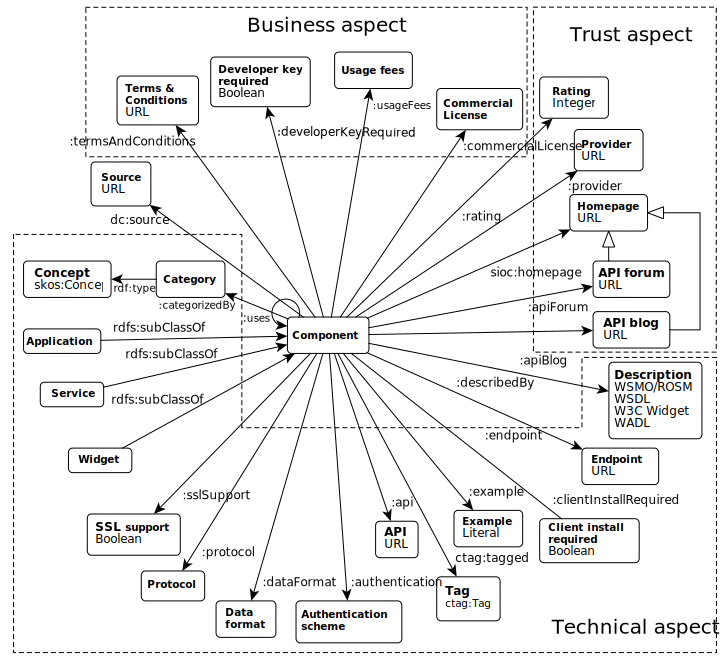
\includegraphics[width=400pt]{graphics/limon.pdf}
	\caption{Omelette mash-up Registry RDF model}
	\label{fig:omeletterdfmodel}
\end{figure}

The registry integrates heterogeneous components that can be potentially used in various web applications. More specifically, mash-up applications and services from the Web are the ones under consideration. mash-up is treated as a first-class object that is comprised of any web applications. Examples of mash-ups and services can be found in repositories such as Yahoo Pipes or Programmable Web.

In order to make these components available for developers, the registry stores relevant metadata that can be used by the developers for selecting components. Additionally, these metadata should be available in the web in order to make it possible to automate the population of the registry with real components. Usually, web component repositories contain metadata such as a component's name, textual description, tags or categorization. Other specific properties that depend on the nature of the component can also be found, such as inputs, endpoints, web service dependencies, or underlying formal descriptions like WSMO or WSDL.

With these considerations in mind, the OMELETTE team has defined the model presented in Figure \ref{fig:omeletterdfmodel}: LiMOn (Linked mash-up Ontology). It is a model that integrates the properties and fields that are provided by current component repositories in the web. Its name comes for its approach of bringing Linked Data to mash-up-Driven Development. It allows describing mash-ups and their components for integrating and sharing mash-up information such as categorization or dependencies.

This model covers aspects such as general categorization metadata, licensing or usage, and basic aspects of component execution. It reuses Simple Knowledge Organization System (SKOS\footnote{http://www.w3.org/2009/08/skos-reference/skos.html}), Friend of a Friend (FOAF\footnote{http://xmlns.com/foaf/spec/}), Dublin Core (DC\footnote{http://dublincore.org/}) and Common Tag (CTag\footnote{ttp://commontag.org/Home}) ontologies in order to follow the guiding principle of Semantic Web, which manifest reusability
as one of the main postulates.

The OMELETTE schema also makes use of work done in SOA4All~\cite{soa4all} FP7 project on RESTful services with ROSM/WSMO service descriptions. Every component might reference an additional description, such as WSDL, WSMO or W3C widget. As shown in the discovery section, ROSM will be used as the basis for describing REST services.

A registry with component descriptions according to the presented model can be queried using a SPARQL query as the one below:

\begin{lstlisting}[style=consola,caption={Example SPARQL}]
PREFIX om: <http://www.ict-omelette.eu/schema.rdf#>
PREFIX ctag: <http://commontag.org/ns#>
PREFIX rdfs: <http://www.w3.org/2000/01/rdf-schema#>

SELECT ?service
WHERE
{ ?service rdf:type om:Service;
	om:categorizedBy om:Telco;
	ctag:tagged [ rdfs:label "video" ];
	ctag:tagged [ rdfs:label "conference" ];
	om:developerKeyRequired "false". }
\end{lstlisting}

This query retrieves telco services with video conferencing functionality. The next SPARQL query asks the registry for services able to search a picture by keywords. It also retrieves the actual endpoint or URL that needs to be accessed to run the service:

\begin{lstlisting}[style=consola,caption={Example SPARQL keywords}]
PREFIX om: <http://www.ict-omelette.eu/schema.rdf#>
PREFIX ctag: <http://commontag.org/ns#>
PREFIX rosm: <http://www.wsmo.org/ns/rosm/0.1#>
PREFIX hrests: <http://www.wsmo.org/ns/hrests#>
PREFIX rdfs: <http://www.w3.org/2000/01/rdf-schema#>

SELECT ?service ?endpoint
WHERE
	{ ?service rdf:type om:Service;
	ctag:tagged
	[ rdfs:label "photos" ];
	om:describedBy [ rdf:type
	rosm:Service;
	rosm:requestURIParemeter [ ctag:tagged [ rdfs:label "keywords" ] ];
	hrests:hasAddress
	?endpoint ]. }
\end{lstlisting}


\section{Automated Discovery}
\label{sec:enableautomated}

Automated discovery is one of the tasks present in the scope of this project. Its objective is to enable OMELETTE users to access a wide amount of web components (i.e. both widgets and services) inside the OMR. Thanks to the automated discovery capabilities OMELETTE users will be able to use services and widgets as soon as they are published on external repositories.


\subsection{Introduction}

Three repositories were mined for services, widgets and mash-ups at this stage of the project,
namely Programmable Web\footnote{http://www.programmableweb.com/}, Opera Widgets\footnote{http://widgets.opera.com/} and Yahoo Pipes\footnote{http://pipes.yahoo.com/}.


\begin{description}
  \item[ProgrammableWeb] \hfill \\
  Programmable Web, shown in \ref{fig:programmableweb}, is the most popular registry of APIs and mash-ups on the Web, and allows developers to include their APIs or mash-ups for other developers. It currently contains more than 3,000 APIs and more than 5,000 mash-ups. Information about which APIs are used by mash-ups, licensing issues, or categorization information can be found in Programmable Web too.

\begin{figure}[ht!]
\centering
\includegraphics[width=400pt]{graphics/programmableweb.png}
\caption{ProgrammableWeb}
\label{fig:programmableweb}
\end{figure}
  
  \item[Yahoo Pipes] \hfill \\
  Yahoo Pipes, shown in \ref{fig:yahopipes}, is a mash-up environment developed by Yahoo, where developers can build data feeds that make use of other feeds by visually dragging and dropping operators and sources. The resulting so-called "pipes" can be run as any other feed, also accepting input parameters and providing a standardized RSS output. The pipes, or mash-ups, are categorized by tags, data format, sources, and also include short textual descriptions.

\begin{figure}[ht!]
\centering
\includegraphics[width=400pt]{graphics/yahoopipes.png}
\caption{Yahoo Pipes}
\label{fig:yahopipes}
\end{figure}

  \item[Opera Widgets] \hfill \\
  Opera Widgets, shown in \ref{fig:operawidgets}, is a repository of mainly W3C widgets that are shared among the community of users of Opera Web Browser. These widgets can be used in OMELETTE because they follow W3C Widget standard. The repository provides a categorized collection of widgets, along with short textual descriptions of the widget's functionality.

\begin{figure}[ht!]
\centering
\includegraphics[width=400pt]{graphics/operawidgets.png}
\caption{Opera Widgets}
\label{fig:operawidgets}
\end{figure}
\FloatBarrier
\end{description}

\subsection{Discovery techniques}
\label{subsec:limonontology}

In order to mine the mentioned websites, a common approach was employed to extract the data. As part of the World Wide Web, the three repositories show a RESTful architecture, where a set of interlinked resources are published with resource specific descriptions. The format of the returned representations of the web resources is not standard, as they do not use any form of semantic annotations on top of the HTML data.

To map the HTML representations of the web resources available in these repositories to the RDF model defined for the OMELETTE mash-up Registry, the Scraping Ontology~\cite{fernandez2011semantic} ~\cite{scont11} has be used by the Open Source screen scraper called Scrappy ~\cite{scr11}, both developed in the context of OMELETTE.

Figure \ref{fig:mappingexample1} shows an example of mapping out of an unstructured HTML document into an OMELETTE RDF graph. In that example, a set of fragments in the HTML page are described along with the RDF data they represent. After processing that information on a particular sample HTML document, a scraper can produce the resulting RDF graph.

\begin{figure}[ht!]
\centering
\includegraphics[width=350pt]{graphics/graph1.png}
\caption{Mapping example for data extraction}
\label{fig:mappingexample1}
\end{figure}

\begin{figure}[ht!]
\centering
\includegraphics[width=350pt]{graphics/graph2.png}
\caption{Mapping example for data extraction}
\label{fig:mappingexample2}
\end{figure}


The methodology followed for the discovery assumes that first of all it is necessary to define a set of mappings for each of the repositories. These mappings state what data could be extracted, and how it could be done. Then prepared mappings are used by Scrappy to crawl the sites and build an RDF knowledge base that is dumped into the OMR.

In the case of Programmable Web, each web resource either represents a mash-up or an API. For each of them, the fields shown are mapped into an element of the ontology, covering the components' metadata such as categorization or tagging.

Similarly, for Opera Widgets each web resource represents a widget, so the information about the widget is mapped to the terms from the ontology. Also, its widget package (which uses WGT extension\footnote{http://www.w3.org/TR/2011/REC-widgets-20110927/}) is mapped as well as the widget's endpoint.

In Yahoo Pipes, more advanced scraping has been performed, thanks to an implicit service description that is available as an HTML form. For each pipe, a form for its execution is available in the mash-up's webpage, as shown in Figure \ref{fig:yahoopipesmash-up}.

\begin{figure}[ht!]
\centering
\includegraphics[width=350pt]{graphics/yahoopipesmashup.png}
\caption{Execution page of a Yahoo Pipe's mash-up}
\label{fig:yahoopipesmash-up}
\end{figure}

These HTML forms are mapped to a Resource-Oriented Service Model (ROSM) or a Web Service Modeling Ontology (WSMO) description in order to get detailed information of the
service's interface. 

\newpage
An example of ROSM description, extracted from the pipe shown in the Figure \ref{fig:mappingexample1}, which accepts a set of textual keywords on a URL, is shown next:


\begin{lstlisting}[style=listXML,caption={Example ROSM definition}]
<rosm:Service>
	<rosm:supportsOperation>
		<rosm:Operation>
			<hrests:hasAddress
			rdf:resource="http://pipes.yahoo.com/pipes/pipe.info?_id=c32fa09"/>
				<rosm:requestURIParameter>
					<rdf:Description>
						<ctag:tagged>
							<rdf:Description>
								<rdfs:label>text</rdfs:label>
							</rdf:Description>
						</ctag:tagged>
						<rdfs:label>keyword</rdfs:label>
				</rdf:Description>
			</rosm:requestURIParameter>
		</rosm:Operation>
	</rosm:supportsOperation>
</rosm:Service>

\end{lstlisting}

\section{Conclusions}

In this chapter we have introduces some of the technologies wich are part of the OMELETTE project and conform the base for this master thesis.

It is necessary to understand first what a repository is for and how the automated discovery is done. We have also introduced the websites scrapped and this helps to understand what kind of services and widgets populate the repository.






\chapter{Requirement Analysis}
\label{chap:requirements}

\begin{chapterintro}
This chapter describes one of the most important stages in software development: the requirement analysis using different scenarios. For this, a detailed analysis of the possible use cases is made using the Unified Modeling Language (UML). This language allows us to specify, build and document a system using graphic language. 
\end{chapterintro}


\cleardoublepage

\section{Overview}
The result of this chapter will be a complete specification of the requirements, which will be matched by each module in the design stage. This helps us also to focus on key aspects and take apart other less important functionalities that could be implemented in future works.

%As commented before, our project aims to develop a personal assistance system that integrates the advantages of agent systems, information retrieval and Natural Language Processing. Our personal assistant should have the capability to solve user's questions using all of these features.

\section{Use cases}

These sections identify the use cases of the system. This helps us to obtain a complete specification of the uses of the system, and therefore define the complete list of requisites to match.  First, we will present a list of the actors in the system and a UML diagram representing all the actors participating in the different use cases. This representation allows, apart from specifying the actors that interact in the system, the relationships between them.

These use cases will be described the next sections, including each one a table with their complete specification. Using these tables, we will be able to define the requirements to be established.


\subsection{Actors dictionary}

\noindent The list of primary and secondary actors is presented in table \ref{tab:actores}. These actors participate in the different use cases, which are presented later.\\



\begin{table}[!htpb]
\centering
\begin{tabular}{|c|c|x{6cm}|}
\noalign{\hrule height 2pt}
\textbf{Actor identifier} & \textbf{Role} & \textbf{Description}\tn
\hline
ACT-1 & User & End user that uses Omelette mash-up Editor  to find a mash-up based on her goals, which are expressed using keywords\tn
\hline
ACT-2 & Developer & Technical developer which uses the OMR.\tn
\hline
ACT-4 & Admin & Administrator of the OMR, in charge of tasks such as inserting, deleting mash-ups, as well as including new available mash-up repositories..\tn
\hline
ACT-5 & MDP & mash-up Delivery Platform, component of the "Live Omelette Environment" that executes mash-ups..\tn
\hline
ACT-6 & External service & External services for executing actions.\tn
\noalign{\hrule height 2pt}
\end{tabular}
\caption{Actors list}
\label{tab:actores}
\end{table}




~\\



\FloatBarrier


\subsection{OMR composition and search use case}
This use case package collects the search functionalities of OMR, as shown in \ref{fig:pack-uc1}.

The use cases presented in this section are as shown in the Figure \ref{fig:pack-uc1}:
\begin{itemize}
\item \textit{keyword search} detailed in sub-section \ref{subsec:keywordsearch}.
\item \textit{mashup browse by category} detailed in sub-section \ref{subsec:mashupbrowsebycat}.
\item \textit{ask question}  detailed in sub-section \ref{subsec:askquestion}.
\item \textit{mashup search by query}  detailed in sub-section \ref{subsec:mashupsearchbyquery}.
\item \textit{mashup compose}  detailed in sub-section \ref{subsec:mashupcompose}.
\end{itemize}


\begin{figure}[h]
\centering
\includegraphics{graphics/uc1.pdf}
\caption{Composition and Search use case}
\label{fig:pack-uc1}
\end{figure}

\newpage
\subsubsection{Keyword search}
\label{subsec:keywordsearch}

\begin{table}[!htpb]
\centering
\begin{tabular}{|c|x{1cm}x{5cm}x{5cm}|}
\noalign{\hrule height 2pt}
\textbf{Use Case Name} & \multicolumn{3}{c|}{keyword search}\\
\hline
\textbf{Use Case ID} & \multicolumn{3}{x{11cm}|}{UC1.1}\\
\hline
\textbf{Pre-Condition} & \multicolumn{3}{x{11cm}|}{OMR  has been fed with  mash-ups and individual services}\\
\hline
\textbf{Post-Condition} & \multicolumn{3}{x{11cm}|}{Optionally, the developer completes the MDL definition to make a mash-up executable}\\
\hline
\textbf{Flow of Events} & \multicolumn{1}{c|}{} & \multicolumn{1}{x{5cm}|}{Actor Input} & \multicolumn{1}{x{5cm}|}{System Response}\\
\hline

\textbf{} & \multicolumn{1}{x{0.5cm}|}{1} & \multicolumn{1}{x{5cm}|}{The user / developer expresses her goals by using textual keywords} & \multicolumn{1}{x{5cm}|}{Ranked result list of mash-ups and individual services. The  mash-up can be an existing  mash-up or a new dynamically composed  mash-up, which can be executable or not. In the same way, the service can be automatically available in the editor or could require human intervention. }\\
\hline

\textbf{} & \multicolumn{1}{x{0.5cm}|}{2a} & \multicolumn{1}{x{5cm}|}{The user / developer access  service / mash-up metadata and   selects one  service / mash-up in order to use it} & \multicolumn{1}{x{5cm}|}{System shows details of the metadata service / mash-up.}\\
\hline

\textbf{} & \multicolumn{1}{x{0.5cm}|}{2b} & \multicolumn{1}{x{5cm}|}{The developer has obtained a non executable  mash-up and opens the editor to complete it} & \multicolumn{1}{x{5cm}|}{The system opens the mash-up editor, which allows the user to finish the mash-up composition (giving API details, etc.), completing the MDL, and finally, publishing the resulting  mash-up in the OMR.}\\
\hline


\end{tabular}
\end{table}

\FloatBarrier


\subsubsection{Mash-up browse by category}
\label{subsec:mashupbrowsebycat}


\begin{table}[!htpb]
\centering
\begin{tabular}{|c|x{1cm}x{5cm}x{5cm}|}
\noalign{\hrule height 2pt}
\textbf{Use Case Name} & \multicolumn{3}{c|}{mash-up browse by category}\\
\hline
\textbf{Use Case ID} & \multicolumn{3}{x{11cm}|}{UC1.2}\\
\hline
\textbf{Primary Actor} & \multicolumn{3}{c|}{User, Developer }\\
\hline
\textbf{Pre-Condition} & \multicolumn{3}{x{11cm}|}{OMR  has been fed with mash-ups and services and has categorized the service / mash-ups according to one or more categories. For example, users can follow a taxonomy based on their needs and types of applications, such as Appstore, while developers can follow a taxonomy based on the technology, integration needs, etc. }\\
\hline
\textbf{Post-Condition} & \multicolumn{3}{x{11cm}|}{-}\\
\hline
\textbf{Flow of Events} & \multicolumn{1}{c|}{} & \multicolumn{1}{x{5cm}|}{Actor Input} & \multicolumn{1}{x{5cm}|}{System Response}\\
\hline

\textbf{} & \multicolumn{1}{x{0.5cm}|}{1} & 
\multicolumn{1}{x{5cm}|}{The user / Developer selects a category} & 
\multicolumn{1}{x{5cm}|}{Ranked list of service / mash-ups belonging to that category}\\
\hline

\textbf{} & \multicolumn{1}{x{0.5cm}|}{2} & 
\multicolumn{1}{x{5cm}|}{The user / developer refines the search with filtering options} & 
\multicolumn{1}{x{5cm}|}{Filtered result set based on filtering options}\\
\hline


\end{tabular}
\end{table}
\FloatBarrier

\newpage
\subsubsection{mash-up search by query}
\label{subsec:mashupsearchbyquery}


\begin{table}[!htpb]
\centering
\begin{tabular}{|c|x{1cm}x{5cm}x{5cm}|}
\noalign{\hrule height 2pt}
\textbf{Use Case Name} & \multicolumn{3}{c|}{mash-up search by query}\\
\hline
\textbf{Use Case ID} & \multicolumn{3}{x{11cm}|}{UC1.3}\\
\hline
\textbf{Primary Actor} & \multicolumn{3}{c|}{Developer}\\
\hline
\textbf{Pre-Condition} & \multicolumn{3}{x{11cm}|}{OMR has been fed with service / mash-ups}\\
\hline
\textbf{Post-Condition} & \multicolumn{3}{x{11cm}|}{-}\\
\hline
\textbf{Flow of Events} & \multicolumn{1}{c|}{} & \multicolumn{1}{x{5cm}|}{Actor Input} & \multicolumn{1}{x{5cm}|}{System Response}\\
\hline

\textbf{} & \multicolumn{1}{x{0.5cm}|}{1} & 
\multicolumn{1}{x{5cm}|}{The developer executes a query using a query language (for example, SPARQL)} & 
\multicolumn{1}{x{5cm}|}{Result set of matching service / mash-ups}\\
\hline


\end{tabular}
\end{table}
\FloatBarrier

\newpage
\subsubsection{mash-up compose}
\label{subsec:mashupcompose}

\begin{table}[!htpb]
\centering
\begin{tabular}{|c|x{1cm}x{5cm}x{5cm}|}
\noalign{\hrule height 2pt}
\textbf{Use Case Name} & \multicolumn{3}{c|}{mash-up compose}\\
\hline
\textbf{Use Case ID} & \multicolumn{3}{x{11cm}|}{UC1.4}\\
\hline
\textbf{Primary Actor} & \multicolumn{3}{c|}{User, developer}\\
\hline
\textbf{Pre-Condition} & \multicolumn{3}{x{11cm}|}{OMR has been fed with individual services and  mash-ups}\\
\hline
\textbf{Post-Condition} & \multicolumn{3}{x{11cm}|}{Optionally, the developer completes the MDL definition to make a mash-up executable}\\
\hline
\textbf{Flow of Events} & \multicolumn{1}{c|}{} & \multicolumn{1}{x{5cm}|}{Actor Input} & \multicolumn{1}{x{5cm}|}{System Response}\\
\hline

\textbf{} & \multicolumn{1}{x{0.5cm}|}{1} & 
\multicolumn{1}{x{5cm}|}{The User / Developer expresses her goals using textual keywords} & 
\multicolumn{1}{x{5cm}|}{Since there is no service mash-up that fulfills the user goals, the system analyses potential combinations of available mash-ups in OMR and provides a composed mash-up or a template of a potential composition}\\
\hline

\end{tabular}
\end{table}
\FloatBarrier

\newpage
\subsubsection{Ask suggestion}
\label{subsec:askquestion}

\begin{table}[!htpb]
\centering
\begin{tabular}{|c|x{1cm}x{5cm}x{5cm}|}
\noalign{\hrule height 2pt}
\textbf{Use Case Name} & \multicolumn{3}{c|}{Ask suggestion}\\
\hline
\textbf{Use Case ID} & \multicolumn{3}{x{11cm}|}{UC1.5}\\
\hline
\textbf{Primary Actor} & \multicolumn{3}{c|}{Editor}\\
\hline
\textbf{Pre-Condition} & \multicolumn{3}{x{11cm}|}{OMR has been fed with individual services and  mash-ups}\\
\hline
\textbf{Post-Condition} & \multicolumn{3}{x{11cm}|}{}\\
\hline
\textbf{Flow of Events} & \multicolumn{1}{c|}{} & \multicolumn{1}{x{5cm}|}{Actor Input} & \multicolumn{1}{x{5cm}|}{System Response}\\
\hline

\textbf{} & \multicolumn{1}{x{0.5cm}|}{1} & 
\multicolumn{1}{x{5cm}|}{The mash-up editor requests a list of available service /   mash-ups to suggest them to the user} & 
\multicolumn{1}{x{5cm}|}{Ranked result list of  service / mash-ups expressed in MDL. The  mash-up can be an existing  mash-up or a new dynamically composed mash-up, which can be executable or not}\\
\hline

\end{tabular}
\end{table}
\FloatBarrier

\newpage
\subsection{OMR discovery and administration use case}
This use case package collects the main administration use cases of the OMR, as shown in \ref{fig:pack-uc2}

\begin{itemize}
\item \textit{automated mash-up feeding} detailed in subsection \ref{subsec:automatedmashupfeeding}
\item \textit{manual mash-up feeding} detailed in subsection \ref{subsec:manualmashupmanagement}
\item \textit{form discovery and description} detailed in subsection \ref{subsec:formdiscoveryanddescription}
\item \textit{mash-up registry integration} detailed in subsection \ref{subsec:mashupregistryintegration}
\item \textit{mash-up registry API based integration} detailed in subsection \ref{subsec:apibasedintegration}
\item \textit{mash-up registry Scrappy based integration} detailed in subsection \ref{subsec:scrappybasedintegration}
\item \textit{manual mash-up management} detailed in subsection \ref{subsec:manualmashupmanagement}
\item \textit{browse pending} detailed in subsection \ref{subsec:pending}
\item \textit{validate service} detailed in subsection \ref{subsec:validate}
\item \textit{reject service} detailed in subsection \ref{subsec:reject}
\end{itemize}

\begin{figure}[h]
\centering
\includegraphics[width=400pt]{graphics/uc2.pdf}
\caption{OMR discovery and administration use case}
\label{fig:pack-uc2}
\end{figure}

\FloatBarrier

\newpage
\subsubsection{Automatic mash-up feeding}
\label{subsec:automatedmashupfeeding}

\begin{table}[!htpb]
\centering
\begin{tabular}{|c|x{1cm}x{5cm}x{5cm}|}
\noalign{\hrule height 2pt}
\textbf{Use Case Name} & \multicolumn{3}{c|}{Automatic mash-up feeding }\\
\hline
\textbf{Use Case ID} & \multicolumn{3}{x{11cm}|}{UC2.1}\\
\hline
\textbf{Primary Actor} & \multicolumn{3}{c|}{Admin}\\
\hline
\textbf{Pre-Condition} & \multicolumn{3}{x{11cm}|}{Availability of external service mash-up repositories or web sites}\\
\hline
\textbf{Post-Condition} & \multicolumn{3}{x{11cm}|}{Service / mash-ups are added to OMR}\\
\hline
\textbf{Flow of Events} & \multicolumn{1}{c|}{} & \multicolumn{1}{x{5cm}|}{Actor Input} & \multicolumn{1}{x{5cm}|}{System Response}\\
\hline

\textbf{} & \multicolumn{1}{x{0.5cm}|}{1} & 
\multicolumn{1}{x{5cm}|}{The admin selects a  mash-up source } & 
\multicolumn{1}{x{5cm}|}{The system connects to the service mash-up source and obtains potential  mash-ups, their metadata, and catalogues them}\\
\hline

\textbf{} & \multicolumn{1}{x{0.5cm}|}{2} & 
\multicolumn{1}{x{5cm}|}{} & 
\multicolumn{1}{x{5cm}|}{he system generates automatically the MDL (partial MDL or  executable MDL).}\\
\hline

\textbf{} & \multicolumn{1}{x{0.5cm}|}{3a} & 
\multicolumn{1}{x{5cm}|}{(Optional) the admin reviews results and approves them for its inclusion in the registry.} & 
\multicolumn{1}{x{5cm}|}{}\\
\hline

\textbf{} & \multicolumn{1}{x{0.5cm}|}{3b} & 
\multicolumn{1}{x{5cm}|}{The discovered mash-ups are automatically integrated in the registry.} & 
\multicolumn{1}{x{5cm}|}{}\\
\hline

\end{tabular}
\end{table}
\FloatBarrier

\newpage
\subsubsection{HTML Form discovery and description}
\label{subsec:formdiscoveryanddescription}

\begin{table}[!htpb]
\centering
\begin{tabular}{|c|x{1cm}x{5cm}x{5cm}|}
\noalign{\hrule height 2pt}
\textbf{Use Case Name} & \multicolumn{3}{c|}{Automatic mash-up feeding }\\
\hline
\textbf{Use Case ID} & \multicolumn{3}{x{11cm}|}{UC2.2}\\
\hline
\textbf{Primary Actor} & \multicolumn{3}{c|}{Admin}\\
\hline
\textbf{Pre-Condition} & \multicolumn{3}{x{11cm}|}{Availability of external web sites offering services}\\
\hline
\textbf{Post-Condition} & \multicolumn{3}{x{11cm}|}{Service / mash-ups are added to OMR}\\
\hline
\textbf{Flow of Events} & \multicolumn{1}{c|}{} & \multicolumn{1}{x{5cm}|}{Actor Input} & \multicolumn{1}{x{5cm}|}{System Response}\\
\hline

\textbf{} & \multicolumn{1}{x{0.5cm}|}{1} & 
\multicolumn{1}{x{5cm}|}{The admin selects a interesting domain and a description schema for that  domain (mash-up metadata). Optionally, the admin selects a set of potential interesting web domain as well as a black list} & 
\multicolumn{1}{x{5cm}|}{The system crawls the web looking for web sites which match  the domain. The system identifies interesting HTML forms, characterizes these HTML forms as well as their results. Then, it classifies the identified mash-up, generates its MDL and adds it to the OMR.}\\
\hline

\textbf{} & \multicolumn{1}{x{0.5cm}|}{2a} & 
\multicolumn{1}{x{5cm}|}{(Optional) the admin reviews the results and approves them for its inclusion in the registry.} & 
\multicolumn{1}{x{5cm}|}{}\\
\hline

\textbf{} & \multicolumn{1}{x{0.5cm}|}{2b} & 
\multicolumn{1}{x{5cm}|}{} & 
\multicolumn{1}{x{5cm}|}{The discovered service / mash-ups are automatically integrated in the registry.}\\
\hline


\end{tabular}
\end{table}
\FloatBarrier

\newpage
\subsubsection{mash-up registry integration}
\label{subsec:mashupregistryintegration}

\begin{table}[!htpb]
\centering
\begin{tabular}{|c|x{1cm}x{5cm}x{5cm}|}
\noalign{\hrule height 2pt}
\textbf{Use Case Name} & \multicolumn{3}{c|}{mash-up registry integration}\\
\hline
\textbf{Use Case ID} & \multicolumn{3}{x{11cm}|}{UC2.3}\\
\hline
\textbf{Primary Actor} & \multicolumn{3}{c|}{Admin}\\
\hline
\textbf{Pre-Condition} & \multicolumn{3}{x{11cm}|}{Availability of external mash-up repositories}\\
\hline
\textbf{Post-Condition} & \multicolumn{3}{x{11cm}|}{mash-ups are added to OMR}\\
\hline
\textbf{Flow of Events} & \multicolumn{1}{c|}{} & \multicolumn{1}{x{5cm}|}{Actor Input} & \multicolumn{1}{x{5cm}|}{System Response}\\
\hline

\textbf{} & \multicolumn{1}{x{0.5cm}|}{1} & 
\multicolumn{1}{x{5cm}|}{The admin selects a mash-up source as well as the polling conditions.} & 
\multicolumn{1}{x{5cm}|}{The system connects to the mash-up source and obtains mash-up descriptions and catalogues them.}\\
\hline

\textbf{} & \multicolumn{1}{x{0.5cm}|}{2a} & 
\multicolumn{1}{x{5cm}|}{(Optional) the admin reviews the results and approves them for its inclusion in the registry.} & 
\multicolumn{1}{x{5cm}|}{}\\
\hline

\textbf{} & \multicolumn{1}{x{0.5cm}|}{2b} & 
\multicolumn{1}{x{5cm}|}{} & 
\multicolumn{1}{x{5cm}|}{The discovered service / mash-ups are automatically integrated in the registry.}\\
\hline


\end{tabular}
\end{table}
\FloatBarrier

\newpage
\subsubsection{API based integration}
\label{subsec:apibasedintegration}

\begin{table}[!htpb]
\centering
\begin{tabular}{|c|x{1cm}x{5cm}x{5cm}|}
\noalign{\hrule height 2pt}
\textbf{Use Case Name} & \multicolumn{3}{c|}{API based integration}\\
\hline
\textbf{Use Case ID} & \multicolumn{3}{x{11cm}|}{UC2.4}\\
\hline
\textbf{Primary Actor} & \multicolumn{3}{c|}{Admin}\\
\hline
\textbf{Pre-Condition} & \multicolumn{3}{x{11cm}|}{Availability of external  mash-up registries offering an API}\\
\hline
\textbf{Post-Condition} & \multicolumn{3}{x{11cm}|}{mash-ups are added to OMR}\\
\hline
\textbf{Flow of Events} & \multicolumn{1}{c|}{} & \multicolumn{1}{x{5cm}|}{Actor Input} & \multicolumn{1}{x{5cm}|}{System Response}\\
\hline

\textbf{} & \multicolumn{1}{x{0.5cm}|}{1} & 
\multicolumn{1}{x{5cm}|}{The admin selects a mash-up source and the polling options.} & 
\multicolumn{1}{x{5cm}|}{The system connects to mash-up source and obtains potential mash-ups, their metadata, and catalogues them}\\
\hline

\textbf{} & \multicolumn{1}{x{0.5cm}|}{2a} & 
\multicolumn{1}{x{5cm}|}{(Optional) the admin reviews the results and approves them for its inclusion in the registry.} & 
\multicolumn{1}{x{5cm}|}{}\\
\hline

\textbf{} & \multicolumn{1}{x{0.5cm}|}{2b} & 
\multicolumn{1}{x{5cm}|}{} & 
\multicolumn{1}{x{5cm}|}{The discovered service / mash-ups are automatically integrated in the registry.}\\
\hline


\end{tabular}
\end{table}
\FloatBarrier

\newpage
\subsubsection{Scraping based integration}
\label{subsec:scrappybasedintegration}

\begin{table}[!htpb]
\centering
\begin{tabular}{|c|x{1cm}x{5cm}x{5cm}|}
\noalign{\hrule height 2pt}
\textbf{Use Case Name} & \multicolumn{3}{c|}{Scraping based integration}\\
\hline
\textbf{Use Case ID} & \multicolumn{3}{x{11cm}|}{UC2.5}\\
\hline
\textbf{Primary Actor} & \multicolumn{3}{c|}{Admin}\\
\hline
\textbf{Pre-Condition} & \multicolumn{3}{x{11cm}|}{Availability of external  mash-up registries  not offering an available API or a restrictive API}\\
\hline
\textbf{Post-Condition} & \multicolumn{3}{x{11cm}|}{mash-ups / Services are added to OMR}\\
\hline
\textbf{Flow of Events} & \multicolumn{1}{c|}{} & \multicolumn{1}{x{5cm}|}{Actor Input} & \multicolumn{1}{x{5cm}|}{System Response}\\
\hline

\textbf{} & \multicolumn{1}{x{0.5cm}|}{1} & 
\multicolumn{1}{x{5cm}|}{The admin selects a mash-up source and defines a description schema} & 
\multicolumn{1}{x{5cm}|}{The system scrapes mash-up registry, obtaining potential  mash-ups / services, and catalogues them}\\
\hline

\textbf{} & \multicolumn{1}{x{0.5cm}|}{2a} & 
\multicolumn{1}{x{5cm}|}{(Optional) the admin reviews the results and approves them for its inclusion in the registry.} & 
\multicolumn{1}{x{5cm}|}{}\\
\hline

\textbf{} & \multicolumn{1}{x{0.5cm}|}{2b} & 
\multicolumn{1}{x{5cm}|}{} & 
\multicolumn{1}{x{5cm}|}{The discovered service / mash-ups are automatically integrated in the registry.}\\
\hline


\end{tabular}
\end{table}
\FloatBarrier

\newpage
\subsubsection{Manual mash-up management}
\label{subsec:manualmashupmanagement}

\begin{table}[!htpb]
\centering
\begin{tabular}{|c|x{1cm}x{5cm}x{5cm}|}
\noalign{\hrule height 2pt}
\textbf{Use Case Name} & \multicolumn{3}{c|}{Manual mash-up management}\\
\hline
\textbf{Use Case ID} & \multicolumn{3}{x{11cm}|}{UC2.6}\\
\hline
\textbf{Primary Actor} & \multicolumn{3}{c|}{Admin}\\
\hline
\textbf{Pre-Condition} & \multicolumn{3}{x{11cm}|}{-}\\
\hline
\textbf{Post-Condition} & \multicolumn{3}{x{11cm}|}{A mash-up is added, deleted to OMR}\\
\hline
\textbf{Flow of Events} & \multicolumn{1}{c|}{} & \multicolumn{1}{x{5cm}|}{Actor Input} & \multicolumn{1}{x{5cm}|}{System Response}\\
\hline

\textbf{} & \multicolumn{1}{x{0.5cm}|}{1a} & 
\multicolumn{1}{x{5cm}|}{The admin selects a  mash-up / service and execute one CRUD operation} & 
\multicolumn{1}{x{5cm}|}{he system executes the operation and returns the result.}\\
\hline

\textbf{} & \multicolumn{1}{x{0.5cm}|}{1b} & 
\multicolumn{1}{x{5cm}|}{(Optional) the system uses filtering options to find the  mash-up (by source, based on properties, etc.)} & 
\multicolumn{1}{x{5cm}|}{}\\
\hline


\end{tabular}
\end{table}
\FloatBarrier

\newpage
\subsubsection{Browse pending mash-ups and services}
\label{subsec:pending}

\begin{table}[!htpb]
\centering
\begin{tabular}{|c|x{1cm}x{5cm}x{5cm}|}
\noalign{\hrule height 2pt}
\textbf{Use Case Name} & \multicolumn{3}{c|}{Browse pending mash-ups and services}\\
\hline
\textbf{Use Case ID} & \multicolumn{3}{x{11cm}|}{UC2.7}\\
\hline
\textbf{Primary Actor} & \multicolumn{3}{c|}{Admin}\\
\hline
\textbf{Pre-Condition} & \multicolumn{3}{x{11cm}|}{OMR has been fed with service / mash-ups}\\
\hline
\textbf{Post-Condition} & \multicolumn{3}{x{11cm}|}{-}\\
\hline
\textbf{Flow of Events} & \multicolumn{1}{c|}{} & \multicolumn{1}{x{5cm}|}{Actor Input} & \multicolumn{1}{x{5cm}|}{System Response}\\
\hline

\textbf{} & \multicolumn{1}{x{0.5cm}|}{1} & 
\multicolumn{1}{x{5cm}|}{The admin filters using facets} & 
\multicolumn{1}{x{5cm}|}{The system executes the corresponding queries and shows the matching mash-ups and services}\\
\hline

\textbf{} & \multicolumn{1}{x{0.5cm}|}{2a} & 
\multicolumn{1}{x{5cm}|}{(Optional) The admin can request at any moment statistics about the filtering} & 
\multicolumn{1}{x{5cm}|}{The system shows the requested statistics using charts}\\
\hline

\textbf{} & \multicolumn{1}{x{0.5cm}|}{2b} & 
\multicolumn{1}{x{5cm}|}{(The admin requests information about a mash-up / service} & 
\multicolumn{1}{x{5cm}|}{The system gets the requested information}\\
\hline


\end{tabular}
\end{table}
\FloatBarrier

\newpage
\subsubsection{Validate a mash-up / service}
\label{subsec:validate}


\begin{table}[!htpb]
\centering
\begin{tabular}{|c|x{1cm}x{5cm}x{5cm}|}
\noalign{\hrule height 2pt}
\textbf{Use Case Name} & \multicolumn{3}{c|}{Validate a mash-up / service}\\
\hline
\textbf{Use Case ID} & \multicolumn{3}{x{11cm}|}{UC2.8}\\
\hline
\textbf{Primary Actor} & \multicolumn{3}{c|}{Admin}\\
\hline
\textbf{Pre-Condition} & \multicolumn{3}{x{11cm}|}{OMR has been fed with service / mash-ups}\\
\hline
\textbf{Post-Condition} & \multicolumn{3}{x{11cm}|}{Services / mash-ups validated into OMR}\\
\hline
\textbf{Flow of Events} & \multicolumn{1}{c|}{} & \multicolumn{1}{x{5cm}|}{Actor Input} & \multicolumn{1}{x{5cm}|}{System Response}\\
\hline

\textbf{} & \multicolumn{1}{x{0.5cm}|}{1} & 
\multicolumn{1}{x{5cm}|}{The admin filters using facets} & 
\multicolumn{1}{x{5cm}|}{The system executes the corresponding queries and shows the matching mash-ups and services}\\
\hline

\textbf{} & \multicolumn{1}{x{0.5cm}|}{2a} & 
\multicolumn{1}{x{5cm}|}{The admin checks the services / mash-ups wanted to be validated} & 
\multicolumn{1}{x{5cm}|}{The system validates the services / mash-ups into OMR}\\
\hline

\end{tabular}
\end{table}
\FloatBarrier

\newpage
\subsubsection{Reject a mash-up / service}
\label{subsec:reject}

\begin{table}[!htpb]
\centering
\begin{tabular}{|c|x{1cm}x{5cm}x{5cm}|}
\noalign{\hrule height 2pt}
\textbf{Use Case Name} & \multicolumn{3}{c|}{Reject a mash-up / service}\\
\hline
\textbf{Use Case ID} & \multicolumn{3}{x{11cm}|}{UC2.9}\\
\hline
\textbf{Primary Actor} & \multicolumn{3}{c|}{Admin}\\
\hline
\textbf{Pre-Condition} & \multicolumn{3}{x{10.5cm}|}{OMR has been fed with service / mash-ups}\\
\hline
\textbf{Post-Condition} & \multicolumn{3}{x{10.5cm}|}{Services / mash-ups rejected into OMR}\\
\hline
\textbf{Flow of Events} & \multicolumn{1}{c|}{} & \multicolumn{1}{x{5cm}|}{Actor Input} & \multicolumn{1}{x{5cm}|}{System Response}\\
\hline

\textbf{} & \multicolumn{1}{x{0.5cm}|}{1} & 
\multicolumn{1}{x{5cm}|}{The admin filters using facets} & 
\multicolumn{1}{x{5cm}|}{The system executes the corresponding queries and shows the matching mash-ups and services}\\
\hline

\textbf{} & \multicolumn{1}{x{0.5cm}|}{2a} & 
\multicolumn{1}{x{5cm}|}{The admin checks the services / mash-ups wanted to be rejected} & 
\multicolumn{1}{x{5cm}|}{The system rejects the services / mash-ups into OMR}\\
\hline

\end{tabular}
\end{table}
\FloatBarrier



\newpage
\subsection{Web interface use case}
This section contains a web interface use case. The client web interface interacts with the OMR in order to obtain consult the registry, which could involve service composition. This use case includes some use cases described previously, as shown in \ref{fig:pack-uc3}.

\begin{itemize}
\item \textit{request available mash-ups} detailed in \ref{subsec:requestavailable}
\item \textit{search mash-ups by query} in \ref{subsec:searchquery}
\item \textit{compose} is not detailed as it is part from the OMELETTE project but not part of this master thesis.
\end{itemize}


\begin{figure}[h]
\centering
\includegraphics[width=400pt]{graphics/uc3.pdf}
\caption{Web interface use case}
\label{fig:pack-uc3}
\end{figure}
\FloatBarrier

\newpage
\subsubsection{Request available mash-ups}
\label{subsec:requestavailable}

\begin{table}[!htpb]
\centering
\begin{tabular}{|c|x{0.5cm}x{5cm}x{5cm}|}
\noalign{\hrule height 2pt}
\textbf{Use Case Name} & \multicolumn{3}{c|}{Request available mash-ups}\\
\hline
\textbf{Use Case ID} & \multicolumn{3}{x{10.5cm}|}{UC3.1}\\
\hline
\textbf{Primary Actor} & \multicolumn{3}{c|}{Web interface}\\
\hline
\textbf{Pre-Condition} & \multicolumn{3}{x{10.5cm}|}{Web interface requests dynamic  mash-up binding}\\
\hline
\textbf{Post-Condition} & \multicolumn{3}{x{10.5cm}|}{Web Interface receives a mash-up list}\\
\hline
\textbf{Flow of Events} & \multicolumn{1}{c|}{} & \multicolumn{1}{x{5cm}|}{Actor Input} & \multicolumn{1}{x{5cm}|}{System Response}\\
\hline

\textbf{} & \multicolumn{1}{x{0.5cm}|}{1a} & 
\multicolumn{1}{x{5cm}|}{Web Interface requests a service / mash-up.} & 
\multicolumn{1}{x{5cm}|}{The system provides a feed with the ranking of available  mash-ups / services.}\\
\hline

\textbf{} & \multicolumn{1}{x{0.5cm}|}{1b} & 
\multicolumn{1}{x{5cm}|}{(Optional) The system does not find a matching service / mash-up and composes a new one on the fly and returns it} & 
\multicolumn{1}{x{5cm}|}{}\\
\hline


\end{tabular}
\end{table}
\FloatBarrier

\newpage
\subsubsection{Search mash-ups by query}
\label{subsec:searchquery}

\begin{table}[!htpb]
\centering
\begin{tabular}{|c|x{0.5cm}x{5cm}x{5cm}|}
\noalign{\hrule height 2pt}
\textbf{Use Case Name} & \multicolumn{3}{c|}{Search mash-ups by query}\\
\hline
\textbf{Use Case ID} & \multicolumn{3}{x{10.5cm}|}{UC3.2}\\
\hline
\textbf{Primary Actor} & \multicolumn{3}{c|}{Web interface}\\
\hline
\textbf{Pre-Condition} & \multicolumn{3}{x{10.5cm}|}{Web interface requests dynamic  mash-up binding}\\
\hline
\textbf{Post-Condition} & \multicolumn{3}{x{10.5cm}|}{Web Interface receives a mash-up list}\\
\hline
\textbf{Flow of Events} & \multicolumn{1}{c|}{} & \multicolumn{1}{x{5cm}|}{Actor Input} & \multicolumn{1}{x{5cm}|}{System Response}\\
\hline

\textbf{} & \multicolumn{1}{x{0.5cm}|}{1a} & 
\multicolumn{1}{x{5cm}|}{Web Interface requests a service / mash-up.} & 
\multicolumn{1}{x{5cm}|}{The system provides a feed with the ranking of available  mash-ups / services.}\\
\hline

\textbf{} & \multicolumn{1}{x{0.5cm}|}{1b} & 
\multicolumn{1}{x{5cm}|}{(Optional) The system does not find a matching service / mash-up and composes a new one on the fly and returns it} & 
\multicolumn{1}{x{5cm}|}{}\\
\hline


\end{tabular}
\end{table}
\FloatBarrier


\subsection{Conclusions}

With the use cases described we have introduced the basic functionalities that have been implemented in this project. They help us to understand the different actors that can interact. They can serve as a base for further development and different use cases that can come to mind. They do not cover mash-up composition, this could be considered for future work lines.

\chapter{Architecture}
\label{chap:architecture}


\begin{chapterintro}
This chapter describes in depth how the system is structured in different modules and how the users interact with them and also how the modules interact with other modules by themselves.
\end{chapterintro}

\cleardoublepage
\section{Architecture Overview}
In this section we will describe the \textbf{videogame architecture}, starting with its two main modules, the \textbf{physical instruments miniatures} and the \textbf{software application}. In Figure \ref{fig:ArchitectureGeneral} we show the global game architecture identifying both main modules and their relation.

\begin{figure}[ht!]
	\centering
	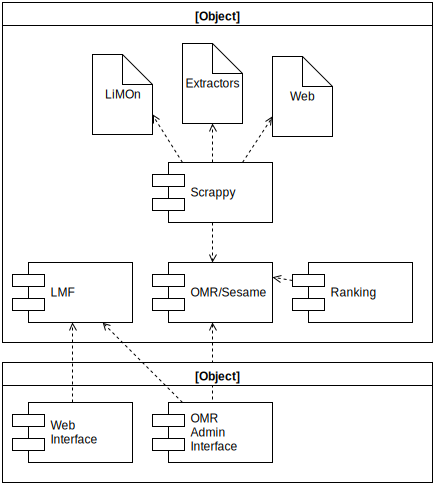
\includegraphics[width=400pt]{graphics/ArchitectureGeneral.pdf}
	\caption{General Architecture}
	\label{fig:ArchitectureGeneral}
\end{figure}

\FloatBarrier

The modules are detailed below:

\subsection{Physical instruments miniatures}
There are five physical miniatures which represents each one of the musical instrument families used at the game: percussion, keyboards, strings, woodwind and brass. The gamer will use these pieces to interact with the app in order to change or activate the family represented by the piece. Also, pieces will be used to access to different game modes.

The interaction between the pieces and the app is haptic, that is, the gamer will pick a miniature and they will place it in the “instrument detection zone” represented by a shiny circle in the app screen. The app “detection algorithm” will determine which piece has been placed and will make an event depending on the game mode and the app state. These events are, for example, changing instrument, activate instrument, etc.

Each piece base has three little pads which conform a triangle used to determine the instrument unequivocally.

Instrument miniatures design will be explain in more detail in section \ref{sec:instrumentminuatures}

\subsection{Application}
The application have been developed using Unity, so we can identify the Unity components included on our app. These components are Unity Scenes, Unity Textures, Unity Assets, Unity Scripts and Unity Sounds. Integrating all of these components into our Unity projects we are able to build the game logic and its graphic interface.

Unity is notable for its ability to target games to multiple platforms. Within a project, we have control over delivery to different mobile devices, web browsers, desktops, and consoles. In our case, we need to develop both Android and iOs applications and Unity allow us to share the same code for them. Also, using Unity Android and iOs Plugins we are able to access to native Android and iOs SDKs, in case we need to access to some Android or iOs native components.

The application archiecture will be explain in more detail in section \ref{sec:application}

\FloatBarrier

\section{Physical instruments miniatures}
\label{sec:instrumentminuatures}
\#Escribir sobre el diseño de los pads en las bases de las piezas para su detección (también sobre el algoritmo de detección)

\FloatBarrier

\section{Application}
\label{sec:application}
The application is the biggest module of the game. It includes the whole software development as it is shown in Figure \ref{fig:applicationarquitecture}.

\begin{figure}[h]
	\centering
	\includegraphics[width=400pt]{graphics/Application_arquitecture.pdf}
	\caption{Application arquitecture diagram}
	\label{fig:applicationarquitecture}
\end{figure}

If we look at the application architecture diagram we can see the Application module where Unity game engine will run. Unity has three main components, Unity Assets, Unity Scripts and Unity Scenes, which are described below:

\subsection{Assets}
An asset is representation of any item that can be used in your game or project. An asset may come from a file created outside of Unity, such as a 3D model, an audio file, an image, or any of the other types of file that Unity supports. There are also some asset types that can be created within Unity, such as an Animator Controller, an Audio Mixer or a Texture Managers. In other words, assets are any resource your game uses.

Thankfully, Unity’s asset importing is robust and intelligent, it will accept all popular 3D file formats and also supports all common image file formats, including PNG, JPEG, TIFF and even layered PSD files directly from Photoshop. When it comes to audio, Unity supports WAV and AIF, ideal for sound effects, and MP3 and OGG for music.

In Figure \ref{fig:applicationarquitecture} we can see that sounds and textures are included as assets to use them, but they are not the only assets we will use. We said that there are some assets types that have been created within Unity to make development easier. In our case we will use an Animation Controller called HOTween, a 2D Texture Manager called 2dToolkit and both Android and iOs plugins. All these assets are included in our Unity project downloading them from Unity Asset Store.

The Unity Asset Store is home to a growing library of free and commercial assets created both by Unity Technologies and also members of the community. A wide variety of assets is available, covering everything from textures, models and animations to whole project examples, tutorials and Editor extensions. These assets are accessed from a simple interface built into the Unity Editor and are downloaded and imported directly into your project.

Assets will be used from the Scenes and/or the Scripts, which are detailed in section \ref{subsec:unityscripts}.

\subsection{Scenes}
Scenes contain the objects of your game. They can be used to create a main menu, individual levels, and anything else. Each unique Scene file as a unique level, where you will place your environments, obstacles, and decorations, essentially designing and building your game in pieces.

We can easily make an analogy between Scenes and screens in our app. Each screen is built from a Scene where all the Assets logic are managed by the Scripts.

Creating Scenes with unity are possible thanks to their intuitive interface, where project assets can be drag to the interface Scene and Scripts can be attached to the assets to control them.

\subsection{Scripts}
\label{subsec:unityscripts}
Scripts, known in Unity as behaviours, let you take assets in your scene and make them interactive. Multiple scripts can be attached to a single object, allowing for easy code reuse. Unity supports three different programming languages; UnityScript, C\#, and Boo. In our project we will use C\#.

As we can see in Figure 3.2, Scripts will manage Unity Assets and will use external Assets from the Unity Asset Store as libraries to make the development easier. In our case, HOTween asset allow us to automate the animation of any numeric (and some non-numeric) property or field (numbers, vectors, transforms, and so on) in many different ways. 2dToolkit provide an efficient 2D sprite, collider set-up and text system which integrates seamlessly into the Unity environment. Android and iOs plugins allow us to access to native Android and iOs libraries.

As we said, scripts will be attached to the scene assets we need to provide them the functionality we need to.


\section{Application use workflow}
The application has three game modes, for each one we will see the application use workflow to get a more precise idea of how the Gamer will interact with the application.

The three game modes were designed as a result of the Game modes use case defined in section \ref{subsec:gamemodes}:

\begin{itemize}
\item \textit{Playing instrument game mode} detailed in sub-section \ref{subsec:playinstrument_arch}.
\item \textit{Conducting orchestra game mode} detailed in sub-section \ref{subsec:conducteorchestra_arch}.
\item \textit{Discovering instrument game mode}  detailed in sub-section \ref{subsec:discoverinstrument_arch}.
\end{itemize}

\newpage
\subsection{Playing instrument game mode}
\label{subsec:playinstrument_arch}

Playing instrument game mode workflow is represented in Figure \ref{fig:playingworkflow}

\begin{figure}[ht!]
	\centering
	\includegraphics[width=400pt]{graphics/PlayingGameMode.pdf}
	\caption{Playing instrument game mode}
	\label{fig:playingworkflow}
\end{figure}

\FloatBarrier

\newpage
\subsection{Conducting orchestra game mode}
\label{subsec:conducteorchestra_arch}

Conducting orchestra game mode workflow is represented in Figure \ref{fig:conductingworkflow}

\begin{figure}[ht!]
	\centering
	\includegraphics[width=400pt]{graphics/ConductingGameMode.pdf}
	\caption{Conducting orchestra game mode}
	\label{fig:conductingworkflow}
\end{figure}

\newpage
\subsection{Discovering instrument game mode}
\label{subsec:discoverinstrument_arch}

Discovering instrument game mode workflow is represented in Figure \ref{fig:discoveringworkflow}

\begin{figure}[ht!]
	\centering
	\includegraphics[width=400pt]{graphics/DiscoveringGameMode.pdf}
	\caption{Discovering instrument game mode}
	\label{fig:discoveringworkflow}
\end{figure}

\FloatBarrier


\section{Conclusions}


\chapter{Prototype and example usage}

\begin{chapterintro}
In this chapter we are going to describe a selected use case. It is going to be explained the running of all the tools involved and its purpose.
It is based on how to crawl the web to find new mashups, then feed the repository, do the validation and rejections of the mashups, and finally the developer will be able to use the discovered services.
\end{chapterintro}

\cleardoublepage

\section{Introduction}

In this use case 2 actors are involved, the administrator and the developer user.

\begin{table}[!htpb]
\centering
\begin{tabular}{|c|c|x{6cm}|}
\noalign{\hrule height 2pt}
\textbf{Actor identifier} & \textbf{Role} & \textbf{Description}\tn
\hline
ACT-1 & Admin & Administrator of the OMR, in charge of tasks such as inserting, deleting mashups, as well as including new available mashup repositories..\tn
\hline
ACT-2 & Developer & Technical developer which uses the OMR.\tn
\noalign{\hrule height 2pt}
\end{tabular}
\caption{Actors list}
\label{tab:actoresusecase}
\end{table}

The goal of the administrator is to provide the user the content that he needs. 

In this context, the developer is building a web application that consists of a social network in which users need to take photos and share them with other users. After sharing them, the photos need to be represented in a map. The developer wants to find an on-line service that already provides this functionality.

The developer user will query the repository using the OMR Web developer interface. The repository must have been fed up previously by an administrator, who doesn't know exactly the services that developers will need but he can think of which might be suitable for them.

To achieve the goals defined before we are going to follow the following steps. First of all launch scrappy to obtain all the web resources we need to feed the repository, once this has been done, the administrator user has to use de OMR admin interface in order to select the mash-ups that the developer user could possibly need for his application. The developer user will be able to find the mash-ups needed using the OMR Web developer interface.

In this scenario each module will run separately to demonstrate that they all can be standalone applications.

There is going to be a remote repository (OMR) located in Chemnitz University of Technology (Germany). The automated discovery process is done using one of the computers in the laboratory of Grupo de Sistemas Inteligentes. Both Administrative interface and developer interface will run in a web server located also in Grupo de Sistemas Inteligentes. The LMF will run in a separated server in the laboratory. This is resumed in table \ref{tab:executionenviroment}.


\begin {table}[h]
\caption {Execution enviroment} \label{tab:executionenviroment} 
\begin{center}
	\begin{tabular}{|c|r|}
		\hline \textbf{Component}                  	   & \textbf{where it runs}          \\ 
		\hline Omelette Mashup Registry (OMR)                  	   &   Chemnitz University of Technology, (Germany)       \\ 
		\hline Automated discovery service                 	   &   Laboratory, GSI (shannon.gsi.dit.upm.es)        \\
		\hline Ranking module 									&   Laboratory, GSI, (shannon.gsi.dit.upm.es)        \\ 
		\hline OMR Administrative interface                 	   &   Laboratory, GSI, (minsky.gsi.dit.upm.es)        \\ 
		\hline OMR Web developer interface                  	   &   Laboratory, GSI, (minsky.gsi.dit.upm.es)        \\
		\hline Linked Media Framework (LMF)                  	   &   Laboratory, GSI, (krusti.gsi.dit.upm.es)        \\ 
		\hline 
	\end{tabular} 
\end{center}
\end{table}

\newpage
\section{Automatic service discovery}
\label{sec:autodiscovery}

As explained in section \ref{sec:scrappy}, the discovery of new services and mashups is done using Scrappy.
Installation and configuration of Scrappy can be found in appendix \ref{apdx:installscrappy}.

The administrator user has to run Scrappy and insert the results into the OMR.
It is important to have configured the OMR endpoint in the config file as explained in appendix \ref{apdx:installscrappy}.

For this example we are going to scrap the sites of \textit{Programable Web}, \textit{Opera Widgets} and \textit{Yahoo Pipes}.

\begin{lstlisting}[style=consola, caption={Scrappy launching}]
scrappy -g programmableweb.com
scrappy -g pipes.yahoo.com
scrappy -g widgets.opera.com
\end{lstlisting}


By executing Scrappy it will directly feed the repository with services in RDF format like listing \ref{lst:fullexamplerdf}.

\begin {table}[h]
\caption {Scrappy execution statistics} \label{tab:scrappyelapsedtime} 
\begin{center}
	\begin{tabular}{|c|c|}
		\hline Elapsed time                  	   & 1 day 3 hours and 31 minutes          \\ 
		\hline 
	\end{tabular} 
\end{center}
\end{table}

\begin {table}[h]
\caption {OMR components summary} \label{tab:omrcomsum} 
\begin{center}
	\begin{tabular}{|c|c|}
		\hline Number of services                  & 10194          \\ 
		\hline Number of widgets                   & 1804           \\ 
		\hline Number of applications              & 7032           \\ 
		\hline \textbf{Total number of components} & \textbf{11998} \\ 
		\hline 
	\end{tabular} 
\end{center}
\end{table}

After the time shown in table \ref{tab:scrappyelapsedtime} the number of mash-ups shown in table \ref{tab:omrcomsum} will be inserted in the repository. In this case we have directly use the OMR, which might have slightly slowed down the process as it needs to do HTTP connections to an external server (and far miles away).

In the figure \ref{fig:programmablewebgoogle} we cam see an example of page that is going to be converted into RDF by Scrappy. In listing \ref{lst:fullexamplerdf} we can see the output that produces Scrappy for that webpage.

\begin{figure}[ht!]
	\centering
	\includegraphics[height=600pt]{graphics/programmable_tags.pdf}
	\caption{Original site and corresponding LiMOn mapping}
	\label{fig:programmablewebgoogle}
\end{figure}

\lstinputlisting[style=listXML, caption=Full RDF of scrapped widget, label={lst:fullexamplerdf}]{code/www_programmableweb_com-api-google-maps.rdf}



\newpage
\section{Ranking algorithm}

The ranking algorithm needs to be executed by the administrator before accessing the OMR admin interface if we want to visualize the metrics corresponding to ranking. It could have done parallel to the scrapping process, but as explained in section \ref{sec:rankingmodule} in order to calculate in an accurate way the ranking indexes all the mash-ups need to be present at the same time because there is correlated information. In the same way, if a new service is discovered by Scrappy because we repeated the process  in section \ref{sec:autodiscovery} we will need to execute the ranking algorithm again.

Before executing the algorithm, it needs to have an instance of Scrappy running as a web server. This is explained in appendix \ref{sec:scrappyusermanual}.

The administrator user has to configure the configuration file configuration.properties (listing \ref{lst:rankingconfigfile}) and the run the algorithm .

\begin{lstlisting}[style=consola,label={lst:runranking}]
bash startRanking.sh
\end{lstlisting}


\begin{lstlisting}[style=consola, label={lst:rankingconfigfile},caption={Ranking algorithm configuration file}]
#OMR endpoint
omr=https://vsr-web.informatik.tu-chemnitz.de/omr-write/components/sparql

#Username
user=omr-client-upm

#Password
password=omr.client.upm.2012
\end{lstlisting}

\begin {table}[h]
\caption {Ranking algorithm execution statistics} \label{tab:rankingelapsedtime} 
\begin{center}
	\begin{tabular}{|c|c|}
		\hline \textbf{Elapsed time}                 	   & 7 hours and 4 minutes          \\ 
		\hline 
	\end{tabular} 
\end{center}
\end{table}

This process could take long time as showed in table \ref{tab:rankingelapsedtime}.

\begin{lstlisting}[style=listXML, label={lst:rdfranking}, caption={Ranking algorithm output}]
<limon:DegCent>0.82</omelette:rating>
<limon:ClosCent>4.21</omelette:rating>
<limon:RatSoc>131</omelette:rating>
\end{lstlisting}

\newpage
\section{OMR administrative interface}

After having the repository filled with all the services our purpose is to select those which we consider as interesting and also reject those which we don't want.
The administrator must enter the administrative interface (see appendix \ref{chap:omradmininstall} for installation and configuration).
In this scenario this is done by opening in the webbrowser the followind URL:
\begin{lstlisting}[style=consola]
http://lab.gsi.dit.upm.es/~pmoncada/omr-admin-pfc
\end{lstlisting}

The administrator will see the main view showed in figure \ref{fig:omradminmainview}.

\begin{figure}[h]
	\centering
	\includegraphics[width=400pt]{graphics/omr-admin-main.png}
	\caption{Main view OMR Administrator}
	\label{fig:omradminmainview}
\end{figure}


In the main view of the OMR Administrator, a menu is shown at the top:

\begin{figure}[h]
	\centering
	\includegraphics[width=200pt]{graphics/admin-top-menu.png}
	\caption{OMR admin top menu}
	\label{fig:topmenuomr}
\end{figure}

\begin{description}
\item[Show approved] shows those mash-ups which have been selected by the
administrator as approved.
\item[Show pending] shows everything that that has been returned has the output of the
scrapping process.
\item[Show rejected] shows the lists of mash-ups that have been previously rejected by
the administrator.
\end{description}

\subsection{Available general actions}
\label{subsec:omravailableactions}
The following options will help the administrator to find those components he thinks of they are interesting or those who might be rejected.

\subsubsection{Filtering}
To filter using the filtering boxes click on a property from a filtering category.
Many filters can be selected at the same time. First select one of them, the view will refresh
with the new results. Then select next filter, the former filter will be sill selected, and results
will be filtered by many filters as chosen.

\textbf{Example}

We want add mash-ups compatible with \textit{JSON and XML } data formats and supporting \textit{REST, JavaScript and HTTP} protocols. To filter the mash-ups with this criteria, we select it in the facet boxes.

\begin{figure}[h]%
    \centering
    \subfloat[limon:protocol]{{\includegraphics[width=4cm]{graphics/limon_protocol.png} }}%
    \qquad
    \subfloat[limon:dataFormat]{{\includegraphics[width=4cm]{graphics/limon_dataformat.png} }}%
    \caption{Filtering by LiMOn properties}%
    \label{fig:limonfiltering}%
\end{figure}

\subsubsection{Searching}
The administrator user can use the search box to find a mash-up by name or description.

\textbf{Example}

We write "maps" in the search box (Figure \ref{fig:omradminsearchbox}), and the results are shown in the result area.

\begin{figure}[h]
	\centering
	\includegraphics[width=100pt]{graphics/maps-search.png}
	\caption{OMR admin search box}
	\label{fig:omradminsearchbox}
\end{figure}

\subsubsection{Obtaining help}
If the administrator does not the meaning of anything appearing in the interface can consult the interactive help by mousing over the help icon.
\begin{figure}[h]
	\centering
	\includegraphics[width=150pt]{graphics/omr-admin-help.png}
	\caption{OMR admin help}
	\label{fig:omradminhelp}
\end{figure}

\subsubsection{Statistics}
\label{subsec:appendixstatistics}

The administrator might know how many mash-ups of a kind are added to the repository. When large amount of services are present is kind of difficult to handle this information. The administrator user can check this information in graphics presentation (Figure ref{fig:omradminseestatistics}).

\begin{figure}[h]
	\centering
	\includegraphics[width=150pt]{graphics/omr-admin-see-statistics.png}
	\caption{OMR see statistics}
	\label{fig:omradminseestatistics}
\end{figure}


\subsection{Reject a resource}

There are several reasons why we would like to reject various discovered mash-ups, such as the functionality of its is not related to our working lines or it was wrong scrapped in the automated discovery process (bad character encoding like in figure \ref{fig:badencoding}, mismatch of the information, etc). We could think just in deleting them from the system, but there is the possibility that we change our mind about this action in the future and we regret it. Also this avoids repeating the scrapping process from re-inserting the mashup again in the repository. This is way the admin interface will allow us to mark the mash-up as rejected as explained in section \ref{subsubsection:validationresourcearch}.

\begin{figure}[h]
	\centering
	\includegraphics[width=400pt]{graphics/omr-bad-encoding.png}
	\caption{Bad charset encoding in widget description}
	\label{fig:badencoding}
\end{figure}

Before validating a resource we may want to know more information about it, and this can be done by visualizing the full content of the service. This must be done before validating, even if we are mostly sure about the component is the desired one, but sometimes as explained in the former paragraph there could be some problems in the scrapped information. The duty of the admin is to make sure the services that are validated are the correct ones.

The administrator can use the tools explained section \ref{subsec:omravailableactions} to get further information and help to complete the process. As an example the administrator could need extra information about the different fields and this can be achieved using the mouse-over functionality.

In our use case we want to have uniform types of mash-ups in the repository so the statistics diagrams provided by the admin interface would result very useful. We can find how to use them in section \ref{subsec:appendixstatistics}.

\subsection{Validating resource example}
As we saw in listing \ref{lst:fullexamplerdf} a service from Google Maps was scrapped, so let's try to find it in the admin interface. The easiest way would be to type "Google Maps API" in the search box and the result would be the desired one. But considering we don't know anything about the scrapped mashup this is not useful. Nevertheless we know some characteristics about a mash-up we need, which are:

\begin{itemize}
	\item It is a widget for maps.
	\item It must be compatible with XML and JSON data format.
	\item It must support javascript.
\end{itemize}

Doing a fast search just writing "maps" in the search box and after this selecting "JSON", "XML" and "Javascript" in the facet boxes the desired result (figure \ref{fig:googlemapsapi} will be showed on the right.

\begin{figure}[h]
	\centering
	\includegraphics[width=400pt]{graphics/google-maps-api.png}
	\caption{Google maps api service in admin interface}
	\label{fig:googlemapsapi}
\end{figure}

To validate this service, the administrator has to click on the check box and then click on the \textit{validate} button to submit the data.

In order to understand the process of validating resources see section \ref{subsubsection:validationresourcearch}.

When we have selected and validated all the services we wanted, our task as administration user will be finished. This task can be resumed at any time if more needed services come out.

\section{Web developer interface}
This application is used by the developer user, who wants to find suitable services to build an application.
It is done using the OMR client interface through the web browser.

\begin{lstlisting}[style=consola,label={lst:runranking}]
http://krusti.gsi.dit.upm.es:8080/omr/
\end{lstlisting}

The interface of this application is much clearer as easier to use than the administrative one, as it is built for end users. Also the functionalities are not exactly the same, in this second search engine there are intelligent technologies as semantic search.

\begin{figure}[h]
	\centering
	\includegraphics[width=400pt]{graphics/omr-client-main.png}
	\caption{OMR Developer interface main}
	\label{fig:searchservice}
\end{figure}


\textbf{Example}

Following the example exposed formerly, a developer wants to embed a map into an application to show the users interesting places. He doesn't know which one will better suit into his requirements. It must be a \textit{widget} and does not want to create a developer account.

The developer user accesses the interface and clicks on the "Search service" button (figure \ref{fig:searchservice}).

\begin{figure}[h]
	\centering
	\includegraphics[width=300pt]{graphics/search-service.png}
	\caption{Search service button}
	\label{fig:searchservice}
\end{figure}

In the next step we can create a new search or select a search (figure \ref{fig:selectsearch}) we did before and we want to reuse it or refine it. The only difference will be that the form in next step will be filled or will be blank.

\begin{figure}[h]
	\centering
	\includegraphics[width=300pt]{graphics/select-search.png}
	\caption{Select saved search or create a new one}
	\label{fig:selectsearch}
\end{figure}

Creating a new search will show us a fillable form which we will fill in according to our search criteria. 

\begin{figure}[h]
	\centering
	\includegraphics[width=400pt]{graphics/omr-client-filters.png}
	\caption{Select filters for the search}
	\label{fig:selectfilters}
\end{figure}

\begin{figure}[h]
	\centering
	\includegraphics[width=300pt]{graphics/omr-client-show-results.png}
	\caption{Show results}
	\label{fig:selectsearch}
\end{figure}


\newpage

And after pressing the "Search results" the semantic search will be done in background by the semantic module and they will be presented as shown in figure \ref{fig:foundservices}. The first three services are marked with \textit{gold}, \textit{silver}, or \textit{bronze} medals which indicate that those are the best 3 services found by the semantic module. At the bottom the developer can see recommended services. These are services ordered by the ranking module having into account the social index.

\begin{figure}[h]
	\centering
	\includegraphics[width=300pt]{graphics/found-services.png}
	\caption{Found services by the semantic module}
	\label{fig:foundservices}
\end{figure}

We can extend the information (figure \ref{fig:extendedinfo}) and check if it satisfies us to finally select it as a candidate to use it in our application.

\begin{figure}[h]
	\centering
	\includegraphics[width=300pt]{graphics/extended-info.png}
	\caption{Extended service info}
	\label{fig:extendedinfo}
\end{figure}

\section{Conclusions}

It is a very powerful search engine that enables real semantic search functionality to the final user, enabling search using natural language and offering similar results that suits into the user preferences that at a first instance he wouldn't have even thinked about.

The setting up of the scenario (filling in the repository and filtering) is quite slow but comparing it to the results given after is more than acceptable. The human intervention of an user administrator to filter the mash-ups gives the final user a great search experience which cannot be done by full automatic search engine of this characteristics.


\chapter{Evaluation}
\label{chap:evaluation}
\begin{chapterintro}
In this chapter we will evaluate the game application through the information retrieved after its deployment
\end{chapterintro}

\cleardoublepage
\section{Overview}
In the following sections we will observe the impact that our application has taken after its deployment. We will analyze both Android and iOs application that we have deployed to Google Play and Apple Store respectively.

The metrics used in this chapter have been recovered using \textit{Game Analytics}. Although ideally we should have used Flurry to retrieved the desired metrics to write this chapter, the client restricted Flurry panel access two years after the application deployment.

Game Analytics is a free and powerful analytics tool for game developers, that helps us to understand player behavior and build better games.~\cite{gametrics1} It is natively included within Unity so we are able to access to lots of metrics out of the box.

\section{Acquisition}

In this section we are going to revise the user acquisition. The most important metrics for user acquisition are number and location of installations. These two metrics are by far the easiest way to tell if our application is something that people find valuable.

We have to notice that although our application is free to download, the pack with the physical instrument pieces should be bought in the client physical stores. This physical pack is shown in Figure \ref{fig:instruments-pack}

\begin{figure}[h]
\centering
\includegraphics[width=350pt]{graphics/evaluation/instruments_pack.jpg}
\caption{Physical instrument pieces box}
\label{fig:instruments-pack}
\end{figure}

This will impact in the application user acquisition due to the fact that our target users will be the ones who have bought the physical game.

\FloatBarrier

We will study the acquisition metrics in two time periods. Firstly, we will look at the information obtained during the first year since the application was first released, this covers the period between August 2014 and August 2015. Then we will observe the information during the three years that the application has been available on the market which covers the period between August 2014 and February 2017.

\subsection{Number of users}

As we said, one of the most important metrics for user acquisition is the number of installations or the number of users which have download our application in their device.

In Figure \ref{fig:bars-first-year} we can see the new users engaged in the first year:

\begin{figure}[h]
\centering
\includegraphics[width=350pt]{graphics/evaluation/bars_users_year.png}
\caption{New users in the first year from release}
\label{fig:bars-first-year}
\end{figure}

As wee can see, we got 2541 users in the first year. Every month the users increased an average of 200 new people. Also, we can observe that there is an evident increase of new users in the months of December and January, which is consequence of the increase of the physical packs sells within Christmas days.

In Figure \ref{fig:bars-all-year} we can see the new users obtained in the whole time our application have been on the market:

\begin{figure}[h]
\centering
\includegraphics[width=350pt]{graphics/evaluation/bars_users_all.png}
\caption{New users since application first release}
\label{fig:bars-all-year}
\end{figure}

\FloatBarrier

As wee can see, we got 4641 users since our application first release. Also, we can observe that after first year new installations have been decreasing with the exception of the Christmas months described earlier. Even so, during 2016 our game has been constantly downloaded by an average of 100 new users.

\subsection{Users location}

Due to the physical instrument pack is sold in the countries list in the Table \ref{tab:countries}, is very useful to observe new user distribution across the world.

\begin{table}[!htpb]
\centering
    \begin{tabular}{|c|c|c|c|c|}
	\hline
	Argentina & Bulgaria & Colombia & Greece & Hungary \\
	\hline
	Israel & Latvia & Mexico & Poland & Qatar \\
	\hline
	Romania & Saudi Arabia & Switzerland & United Arab Emirates & Uruguay \\
	\hline
	Azerbaijan & China & France & Holland & ~\\
	\hline
	Italy & Lithuania & Peru & Portugal & ~\\
	\hline
	Russia & Spain & Turkey & United States & ~\\
    \hline
    \end{tabular}
\caption{Countries were the physical instrument pack is sold}
\label{tab:countries}
\end{table}

\FloatBarrier

In Figure \ref{fig:map-first-year} we can see the world distribution map of users engaged in the first year:

\begin{figure}[h]
\centering
\includegraphics[width=350pt]{graphics/evaluation/map_users_year.png}
\caption{New users location in the first year from release}
\label{fig:map-first-year}
\end{figure}

Also, in Figure \ref{fig:chart-first-year} we can observe the top four countries where the game have been downloaded within this period:

\begin{figure}[h]
\centering
\includegraphics[width=200pt]{graphics/evaluation/chart_users_year.png}
\caption{New users location in the first year from release top countries}
\label{fig:chart-first-year}
\end{figure}

\FloatBarrier

As we can see, the application have been installed from most of the countries located in Europe and America, as long as many countries located in Asia. Also, Spain, Russia, USA and Italy are the countries where most of the users came from.

In Figure \ref{fig:map-all-year} we can see the world distribution map of users obtained in the whole time our application have been on the market:

\begin{figure}[h]
\centering
\includegraphics[width=350pt]{graphics/evaluation/map_users_year.png}
\caption{New users location since application first release}
\label{fig:map-all-year}
\end{figure}

Also, in Figure \ref{fig:chart-all-year} we can observe the top four countries where the game have been downloaded within this period:

\begin{figure}[h]
\centering
\includegraphics[width=200pt]{graphics/evaluation/chart_users_year.png}
\caption{New users location since application first release top countries}
\label{fig:chart-all-year}
\end{figure}

\FloatBarrier

As we can see, the application have been installed from a few more countries from the ones in the first year. Also, Spain, Russia, USA and Italy are the countries where most of the users came from.

\section{Engagement}

Mobile engagement is the act of engaging a user through available messaging channels inside and outside of an app. Because of that, engagement is such an important metric to analyze if the gamer has considered our application useful as their keep using it.

We will observe user engagement since our game is in the market and through two principal blocks of metrics, user retention and DAU, WAU and MAU metrics.

\subsection{Retention}
Retention is arguably the most important metric in a free-to-play game. Successful free-to-play games create long-term relationships with users. Users that enjoy the experience enough are willing to pay to for a competitive advantage. A game needs to have strong retention to have time to build this relationship.

To calculate retention, separate your users into cohorts based on the day they download your app. The day that the download occurs is Day 0. If a user opens your app the next day (Day 1), they are marked as retained. If they do not open the app, they are not retained. This calculation is performed for user cohort on each day after they download the app. Common days used for retention are 1, 3, 7 and 30.~\cite{gametrics2}

In Figure \ref{fig:app-retention} we can see our game 90 day retention since its release:

\begin{figure}[h]
\centering
\includegraphics[width=350pt]{graphics/evaluation/app_retention.png}
\caption{Application retention}
\label{fig:app-retention}
\end{figure}

\FloatBarrier

As we can see, our game retention is 18.18\%. Usually, game applications tend to have lower retention values, and  according to Flurry studies, 8\% retention rate at 30 days is average across the kids game iOs sub-category applications.~\cite{flurry2} In our case, we have duplicate generally retention rates for our type of application.

\subsection{DAU, WAU and MAU}

Daily Active Users (DAUs) is the number of unique users that start at least one session in your app on any given day. By themselves, DAU and other high level metrics don’t provide much insight into an app’s performance. However, knowing these simple metrics is a useful starting point for an educated analytics discussion.

Weekly Active Users (WAUs) is the number of unique users that start at least one session in your app on any given week. Having both DAU and WAU, we can obtain the ratio of Daily Active Users to Weekly Active Users.

Monthly Active Users (MAUs) is the number of unique users that start at least one session in your app on any given month. Having both DAU and MAU, we can obtain the ratio of Daily Active Users to Monthly Active Users shows how well an app retains users and is often referred to as the stickiness of a game. This metric shows you how frequently users log in to your app.

Popular social networking apps like Facebook have reported DAU/MAU ratios as high as 50 percent. But most successful gaming apps have ratios closer to 20 percent.~\cite{gametrics2}

In Figure \ref{fig:app-dau} we can see our DAU, WAU and MAU data:

\begin{figure}[h]
\centering
\includegraphics[width=350pt]{graphics/evaluation/app_dau.png}
\caption{Application retention}
\label{fig:app-dau}
\end{figure}

\FloatBarrier

As we can see, if we calculate the DAU/WAU and DAU/MAU ratios, we obtain 20\% and 6\%. This means that the average user logged in on roughly 6 percent of the days that month.

\subsection{Quality}

We will study our game quality in terms of the average numbers of screens the levels plays and in the average of frames per second their devices give.

In Figure \ref{fig:app-levels} we can see the mean of levels that our gamers plays in every month since the application release.

\begin{figure}[h]
\centering
\includegraphics[width=250pt]{graphics/evaluation/app_levels.png}
\caption{Application levels average}
\label{fig:app-levels}
\end{figure}

\FloatBarrier

As we can see, gamers plays an average of 20 levels per month. In our case, each screen is a level, so the gamer plays thorough at least 20 different screens each month.

Finally, in Figure \ref{fig:app-fps} we can observe the average frames per second shown by gamers devices. 

\begin{figure}[h]
\centering
\includegraphics[width=250pt]{graphics/evaluation/app_fps.png}
\caption{Application fps average}
\label{fig:app-fps}
\end{figure}

\FloatBarrier

As we can see, gamers devices shown an average of 29 frames per second, which is the estimated value for a game which manages lots of audio and animation resources.

\subsection{Summary}
In this chapter we evaluated our application using the metrics available from Unity Game Analytics.

Firstly, we observe user acquisition in order to study the numbers of new users we obtained during the first year of the application in the market and since its release. Also, we took a look at the users location distribution.

Secondly, we detailed user engagement so that we can know if the users tend to use our game after its installation. We took a look at retention information since application release as long as DAU, WAU and MAU metrics.

Finally, we observed the game quality detailed the numbers of levels the gamer played and the numbers of frames per second their devices shown since the application release.



\chapter{Conclusions}
\label{chap:conclusions}
\begin{chapterintro}
In this chapter we will describe the conclusions extracted from this master thesis and detail the achieved goals. Also, the thinkings about future work will be detailed.
\end{chapterintro}

\cleardoublepage
\section{Conclusions}

By using Unity3D as the base to build the application we have been able to create a cross-platform mobile game without the effort requires to manage separate developments for each platform.

We have built an application from scratch following a typical mobile application development lifecycle defined the in the following four different phases: discovery, design, development, testing and deployment.~\cite{vithani2014mod}

Firstly, we covered the requirement analysis phase, determining the needs for our application, taking account of the possibly conflicting requirements of our client, analyzing, documenting, validating and managing software or system requirements.~\cite{kotonya1998requirements}

Secondly, we obtained the use cases, which covers all the functional requirements obtained in the first stage of our development.

Then, we design the game architecture, where we decided to use Unity3D as our game base engine. Moreover, four asset plugins placed in Unity3D (2D Toolkit, HOTween, iOs native and Android native) where included in the architecture in order to improve performance and make the development easier. Also we need to design physical pieces to let the gamer interact with the software application. This pieces have a unique base pads distribution to let our algorithm identify each piece.

Finally, we design three game modes to cover the use cases presented. In this document we have presented two of them.

Following this path we have been able to build a multi-platform mobile musical training software for children using the framework Unity3D engine.

\section{Achieved goals}

In this section we will detail our application's achieved goals checking if we have covered all the use cases presented in section \ref{subsec:gamemodes} 

\begin{description}
\item[Play an instrument]
This goal has been achieved successfully. This use case is described in \ref{subsec:playinstrument}. The gamer is able to play five different instruments, one of each musical instrument family. In order to select the instrument to play with, the gamer is able to place the physical miniature, which represents the instrument family, on a recognition zone in the screen. Also, the gamer can watch a demo or change the melody to be played. We can see this achievement in figures \ref{fig:playing_xylo_start_screen}, \ref{fig:playing_piano_screen}, \ref{fig:playing_harp_screen}, \ref{fig:playing_panpipes_screen} and \ref{fig:playing_trombone_screen}

\item[Conduct the orchestra]
This goal has been achieved successfully. This use case is described in \ref{subsec:conductorchestra}. The gamer is able to conduct the orchestra that is playing the selected melody. The gamer can conduct the melody by enabling or disabling the instruments that are playing this melody. In order to select the instrument family whose instruments will be able to be enabled or disabled, the gamer is able to place the physical miniature, which represents the instrument family, on a recognition zone in the screen. Also, the gamer can watch stop or change the melody to be conducted. We can see this achievement in figures \ref{fig:conducting_all_stop_screen} and \ref{fig:conducting_some_screen}.

\item[Discover an instrument]
This goal has been achieved successfully. This use case is described in \ref{subsec:discoverinstrument}. The gamer is able to read information of instruments of the five different musical families. In order to select the instruments to discover, the gamer is able to place the physical miniature, which represents the instrument family, on a recognition zone in the screen. Also the gamer can reproduce the instrument selected sound. We can see this achievement in figures shown in section \ref{sec:discoveringscreens}

\item[Watch a melody play demo]
This goal has been achieved successfully. This use case is described in \ref{subsec:watchdemo}. Gamer is able to watch a demo of all available melodies in the \textit{Play instrument} game mode with each of the five instruments the gamer is able to play with.

\item[Select a melody]
This goal has been achieved successfully. This use case is described in \ref{subsec:selectmelody}. Gamer is able to select a melody within both \textit{Play instrument} and \textit{Conduct orchestra} game modes.  We can see this achievement in figures \ref{fig:melodies_playing_screen} and \ref{fig:conducting_melodies_screen}.

\item[Select an instrument]
This goal has been achieved successfully. This use case is described in \ref{subsec:selectinstrument}. As we have said in the previous achievements, the gamer is able to choose an instrument within all game modes. In order to select the instrument, the gamer is able to place the physical miniature, which represents the instrument family, on a recognition zone in the screen.

\end{description}

\section{Future work}

There are several lines than can be followed to continue and extend features of this work.

In the following points we present some improvements that we can add to our application to continue the development.

\begin{itemize}
\item Add new instruments to the \textit{Play instrument game mode}. This new feature imply the development of new screens for each new instruments and the manage of new musical sounds.
\item Add new instrument families to the game. This feature imply the design of new pieces as long as modifying the recognition algorithm to support them. Also, the three game modes should be adapted to represent the new instrument families.
\item Update game project to Unity 5. This involves some work related with all Unity components. While many areas are upgraded automatically, there are certain parts of the project where we will need to manually adjust or refactor.
\item Reduce artifacts size. While Android and iOs markets allow us to upload huge sized applications, this suppose that user should only install the application when they are connected through WiFi. This would suppose a barrier to attract new gamers, so artifact size should be reduced from 300 MB, its actual size.
\item Add notifications management system in order to allow the client to interact with the gamer. This would let the client to promote their other applications and the new game features
\item Reduce resources requirements. This would permit lower resources devices to run the application and decrease the battery use.
\item Automate the deployment phase. This feature would allow us to decrease times when applying bug fixes to our application.
\end{itemize}



\appendix
\cleardoublepage
\chapter{Game Play images}

This appendix shows game play captures. It goes through the three different game modes and shows how the gamer interacts with them using the physical instrument pieces.

\cleardoublepage

\section{Playing game mode}

\begin{figure}[ht!]
  \centering
  \includegraphics[width=350pt]{graphics/game-play/enter_playing_mode.png}
  \vspace{0.05cm}
  \caption{Entering playing game mode from home screen}
  \vspace{1cm}

  \includegraphics[width=350pt]{graphics/game-play/playing_piano_free.png}
  \vspace{0.05cm}
  \caption{Playing piano free mode}
\end{figure}

\begin{figure}[ht!]
  \centering
  \includegraphics[width=350pt]{graphics/game-play/choose_melody_playing.png}
  \vspace{0.05cm}
  \caption{Opening melodies menu in playing game mode}
  \vspace{1cm}

  \includegraphics[width=350pt]{graphics/game-play/change_melody_playing.png}
  \vspace{0.05cm}
  \caption{Changing melody to be played in playing game mode}
\end{figure}

\begin{figure}[ht!]
  \centering
  \includegraphics[width=350pt]{graphics/game-play/select_guided_mode.png}
  \vspace{0.05cm}
  \caption{Starting guided playing mode}
  \vspace{1cm}

  \includegraphics[width=350pt]{graphics/game-play/playing_piano_guided.png}
  \vspace{0.05cm}
  \caption{Playing piano guided}
\end{figure}

\begin{figure}[ht!]
  \centering
  \includegraphics[width=350pt]{graphics/game-play/change_strings_playing.png}
  \vspace{0.05cm}
  \caption{Placing strings piece in playing game mode}
  \vspace{1cm}

  \includegraphics[width=350pt]{graphics/game-play/change_woodwind_playing.png}
  \vspace{0.05cm}
  \caption{Placing woodwind piece in playing game mode}
\end{figure}

\begin{figure}[ht!]
  \centering
  \includegraphics[width=350pt]{graphics/game-play/change_brass_playing.png}
  \vspace{0.05cm}
  \caption{Placing brass piece in playing game mode}
  \vspace{1cm}

  \includegraphics[width=350pt]{graphics/game-play/change_percussion_playing.png}
  \vspace{0.05cm}
  \caption{Placing percussion piece in playing game mode}
\end{figure}

\section{Conducting game mode}

\begin{figure}[ht!]
  \centering
  \includegraphics[width=350pt]{graphics/game-play/enter_conducting_mode.png}
  \vspace{0.05cm}
  \caption{Entering conducting game mode from home screen}
  \vspace{1cm}

  \includegraphics[width=350pt]{graphics/game-play/choose_melody_conducting.png}
  \vspace{0.05cm}
  \caption{Opening melodies menu in playing game mode}
\end{figure}

\begin{figure}[ht!]
  \centering
  \includegraphics[width=350pt]{graphics/game-play/change_melody_conducting.png}
  \vspace{0.05cm}
  \caption{Changing melody to be played in playing game mode}
  \vspace{1cm}

  \includegraphics[width=350pt]{graphics/game-play/activate_keyboards_family.png}
  \vspace{0.05cm}
  \caption{Activating keyboards family}
\end{figure}

\begin{figure}[ht!]
  \centering
  \includegraphics[width=350pt]{graphics/game-play/disable_instrument_conducting.png}
  \vspace{0.05cm}
  \caption{Disabling instrument}
  \vspace{1cm}

  \includegraphics[width=350pt]{graphics/game-play/enable_instrument_conducting.png}
  \vspace{0.05cm}
  \caption{Enabling instrument}
\end{figure}

\section{Discovering game mode}

\begin{figure}[ht!]
  \centering
  \includegraphics[width=350pt]{graphics/game-play/enter_discovering_mode.png}
  \vspace{0.05cm}
  \caption{Entering discovering game mode from home screen}
  \vspace{1cm}

  \includegraphics[width=350pt]{graphics/game-play/instrument_sound_discovering.png}
  \vspace{0.05cm}
  \caption{Playing instrument sound}
\end{figure}

\begin{figure}[ht!]
  \centering
  \includegraphics[width=350pt]{graphics/game-play/change_family_discovering.png}
  \vspace{0.05cm}
  \caption{Changing family in discovering game mode}
  \vspace{1cm}

  \includegraphics[width=350pt]{graphics/game-play/change_instrument_discovering.png}
  \vspace{0.05cm}
  \caption{Changing instrument in discovering game mode}
\end{figure}


\cleardoublepage
\chapter{Application game screens}

This appendix shows all the screens which conform the application. It goes through the three different game modes and shows all the screens contained within them.

\cleardoublepage

\section{Home}

\begin{figure}[ht!]
  \centering
  \includegraphics[width=350pt]{graphics/use-case/home_screen.jpg}
  \vspace{0.05cm}
  \caption{Application Home Screen}
  \vspace{0.6cm}

  \includegraphics[width=350pt]{graphics/use-case/help_home_screen.jpg}
  \vspace{0.05cm}
  \caption{Help Home Screen}
\end{figure}

\section{Playing game mode}

\begin{figure}[ht!]
  \centering
  \includegraphics[width=350pt]{graphics/use-case/playing_xylo_start_screen.jpg}
  \vspace{0.05cm}
  \caption{Xylophone playing instrument game mode}
  \vspace{0.6cm}

  \includegraphics[width=350pt]{graphics/use-case/help_playing_screen.jpg}
  \vspace{0.05cm}
  \caption{Help information playing instrument game mode}
\end{figure}

\begin{figure}[ht!]
  \centering
  \includegraphics[width=350pt]{graphics/use-case/playing_panpipes_screen.jpg}
  \vspace{0.05cm}
  \caption{Playing panpipes screen}
  \vspace{0.6cm}

  \includegraphics[width=350pt]{graphics/use-case/playing_trombone_screen.jpg}
  \vspace{0.05cm}
  \caption{Playing trombone screen}
\end{figure}

\begin{figure}[ht!]
  \centering
  \includegraphics[width=350pt]{graphics/use-case/playing_piano_screen.jpg}
  \vspace{0.05cm}
  \caption{Playing piano screen}
  \vspace{0.6cm}

  \includegraphics[width=350pt]{graphics/use-case/playing_harp_screen.jpg}
  \vspace{0.05cm}
  \caption{Playing harp screen}
\end{figure}

\section{Conducting game mode}

\begin{figure}[ht!]
  \centering
  \includegraphics[width=350pt]{graphics/use-case/conducting_home_screen.jpg}
  \vspace{0.05cm}
  \caption{Conducting game mode access screen}
  \vspace{0.6cm}

  \includegraphics[width=350pt]{graphics/use-case/help_conducting_screen.jpg}
  \vspace{0.05cm}
  \caption{Help information conducting orchestra game mode}
\end{figure}

\begin{figure}[ht!]
  \centering
  \includegraphics[width=350pt]{graphics/use-case/conducting_melodies_screen.jpg}
  \vspace{0.05cm}
  \caption{Melodies selection in the conducting orchestra game mode}
  \vspace{0.6cm}

  \includegraphics[width=350pt]{graphics/use-case/conducting_all_stop_screen.jpg}
  \vspace{0.05cm}
  \caption{Conducting orchestra screen with all instruments activated}
\end{figure}

\section{Discovering game mode}
\label{sec:discoveringscreens}

\begin{figure}[ht!]
  \centering
  \includegraphics[width=350pt]{graphics/additional-screens/help_discovering_screen.jpg}
  \vspace{0.05cm}
  \caption{Help Discovering Screen}
  \vspace{0.6cm}

  \includegraphics[width=350pt]{graphics/additional-screens/discovering_perc_drum_screen.jpg}
  \vspace{0.05cm}
  \caption{Discovering drum instrument}
\end{figure}

\begin{figure}[ht!]
  \centering
  \includegraphics[width=350pt]{graphics/additional-screens/discovering_perc_kettle_screen.jpg}
  \vspace{0.05cm}
  \caption{Discovering kettle instrument}
  \vspace{0.6cm}

  \includegraphics[width=350pt]{graphics/additional-screens/discovering_perc_cymbals_screen.jpg}
  \vspace{0.05cm}
  \caption{Discovering cymbals instrument}
\end{figure}

\begin{figure}[ht!]
  \centering
  \includegraphics[width=350pt]{graphics/additional-screens/discovering_perc_xylophone_screen.jpg}
  \vspace{0.05cm}
  \caption{Discovering xylophone instrument}
  \vspace{0.6cm}

  \includegraphics[width=350pt]{graphics/additional-screens/discovering_perc_marimba_screen.jpg}
  \vspace{0.05cm}
  \caption{Discovering marimba instrument}
\end{figure}

\begin{figure}[ht!]
  \centering
  \includegraphics[width=350pt]{graphics/additional-screens/discovering_perc_vibraphone_screen.jpg}
  \vspace{0.05cm}
  \caption{Discovering vibraphone instrument}
  \vspace{0.6cm}

  \includegraphics[width=350pt]{graphics/additional-screens/discovering_brass_trumpet_screen.jpg}
  \vspace{0.05cm}
  \caption{Discovering trumpet instrument}
\end{figure}

\begin{figure}[ht!]
  \centering
  \includegraphics[width=350pt]{graphics/additional-screens/discovering_brass_french_horn_screen.jpg}
  \vspace{0.05cm}
  \caption{Discovering French horn instrument}
  \vspace{0.6cm}

  \includegraphics[width=350pt]{graphics/additional-screens/discovering_brass_trombone_screen.jpg}
  \vspace{0.05cm}
  \caption{Discovering trombone instrument}
\end{figure}

\begin{figure}[ht!]
  \centering
  \includegraphics[width=350pt]{graphics/additional-screens/discovering_brass_tuba_screen.jpg}
  \vspace{0.05cm}
  \caption{Discovering tuba instrument}
  \vspace{0.6cm}

  \includegraphics[width=350pt]{graphics/additional-screens/discovering_brass_flugelhorn_screen.jpg}
  \vspace{0.05cm}
  \caption{Discovering flugelhorn instrument}
\end{figure}

\begin{figure}[ht!]
  \centering
  \includegraphics[width=350pt]{graphics/additional-screens/discovering_key_piano_screen.jpg}
  \vspace{0.05cm}
  \caption{Discovering piano instrument}
  \vspace{0.6cm}

  \includegraphics[width=350pt]{graphics/additional-screens/discovering_key_celesta_screen.jpg}
  \vspace{0.05cm}
  \caption{Discovering celesta instrument}
\end{figure}

\begin{figure}[ht!]
  \centering
  \includegraphics[width=350pt]{graphics/additional-screens/discovering_key_organ_screen.jpg}
  \vspace{0.05cm}
  \caption{Discovering organ instrument}
  \vspace{0.6cm}

  \includegraphics[width=350pt]{graphics/additional-screens/discovering_key_clavichord_screen.jpg}
  \vspace{0.05cm}
  \caption{Discovering clavichord instrument}
\end{figure}

\begin{figure}[ht!]
  \centering
  \includegraphics[width=350pt]{graphics/additional-screens/discovering_strings_violin_screen.jpg}
  \vspace{0.05cm}
  \caption{Discovering violin instrument}
  \vspace{0.6cm}

  \includegraphics[width=350pt]{graphics/additional-screens/discovering_strings_double_bass_screen.jpg}
  \vspace{0.05cm}
  \caption{Discovering double bass instrument}
\end{figure}

\begin{figure}[ht!]
  \centering
  \includegraphics[width=350pt]{graphics/additional-screens/discovering_strings_viola_screen.jpg}
  \vspace{0.05cm}
  \caption{Discovering viola instrument}
  \vspace{0.6cm}

  \includegraphics[width=350pt]{graphics/additional-screens/discovering_strings_chello_screen.jpg}
  \vspace{0.05cm}
  \caption{Discovering chello instrument}
\end{figure}

\begin{figure}[ht!]
  \centering
  \includegraphics[width=350pt]{graphics/additional-screens/discovering_strings_lute_screen.jpg}
  \vspace{0.05cm}
  \caption{Discovering lute instrument}
  \vspace{0.6cm}

  \includegraphics[width=350pt]{graphics/additional-screens/discovering_strings_guitar_screen.jpg}
  \vspace{0.05cm}
  \caption{Discovering guitar instrument}
\end{figure}

\begin{figure}[ht!]
  \centering
  \includegraphics[width=350pt]{graphics/additional-screens/discovering_strings_harp_screen.jpg}
  \vspace{0.05cm}
  \caption{Discovering harp instrument}
  \vspace{0.6cm}

  \includegraphics[width=350pt]{graphics/additional-screens/discovering_wind_flute_screen.jpg}
  \vspace{0.05cm}
  \caption{Discovering flute instrument}
\end{figure}

\begin{figure}[ht!]
  \centering
  \includegraphics[width=350pt]{graphics/additional-screens/discovering_wind_clarinet_screen.jpg}
  \vspace{0.05cm}
  \caption{Discovering clarinet instrument}
  \vspace{0.6cm}

  \includegraphics[width=350pt]{graphics/additional-screens/discovering_wind_oboe_screen.jpg}
  \vspace{0.05cm}
  \caption{Discovering oboe instrument}
\end{figure}

\begin{figure}[ht!]
  \centering
  \includegraphics[width=350pt]{graphics/additional-screens/discovering_wind_bassoon_screen.jpg}
  \vspace{0.05cm}
  \caption{Discovering bassoon instrument}
  \vspace{0.6cm}

  \includegraphics[width=350pt]{graphics/additional-screens/discovering_wind_piccolo_screen.jpg}
  \vspace{0.05cm}
  \caption{Discovering piccolo instrument}
\end{figure}

\begin{figure}[ht!]
  \centering
  \includegraphics[width=350pt]{graphics/additional-screens/discovering_wind_panpipes_screen.jpg}
  \vspace{0.05cm}
  \caption{Discovering panpipes instrument}
\end{figure}



\phantomsection
\addcontentsline{toc}{chapter}{Bibliography}
\bibliographystyle{ieeetr}
{
\small
\bibliography{biblio/ref}
}
\cleardoublepage
\end{document}